\chapter{Characterization of the phase plate}
The final goal of this project was to have a complete characterization of the phase plate that we received from the company Holoor. We knew its expected behaviour, namely the creation of a top hat potential with the characteristics described in \Cref{sec:slm_specifications}. However, it was important to test it to see how it behaved in reality. In this chapter, we will discuss the experimental setup and the methods used in the characterization, especially focusing on the quantities we defined to quantify the \enquote{goodness} of the result. Then, we will discuss the results highlighting the most important aspects to use the phase plate optimally.

\section{Building the experimental setup}
\subsection{Imaging system}
In order to characterize the phase plate, the first step was to set up an imaging system. This was necessary to acquire images of the final intensity distribution. Since the expected dimensions of the intensity distribution were of the order of \SI{10}{\micro\meter}, a magnification system was assembled. The imaging system was composed of a microscope objective, which magnified the beam, and by a camera. The distance between the two was kept constant by fixing them on a cage. The objective could be moved in the horizontal ($y$) and vertical ($z$) direction by turning two micrometers. The whole system (objective and camera) was mounted on a linear translation stage. The stage could be moved along the $x$ direction to focus the image. A sketch of the setup is shown in \cref{fig:imaging}.

\begin{figure}
    \centering
    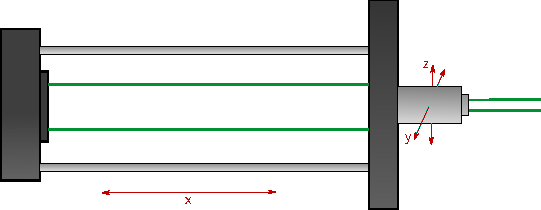
\includegraphics[width=0.65\textwidth]{chapters/chapter_3/figures/imaging}
    \caption{Imaging system. A microscope objective magnifies the image and a CCD camera acquires it. The objective can be moved in the $y$ and $z$ direction with two micrometers. The whole system can be moved in the $x$ direction to focus the image.}
    \label{fig:imaging}
\end{figure}

In order to use the imaging system to take measurements, it had to be calibrated. For the calibration, a laser beam was sent onto a target like the one shown in \cref{fig:target} and imaged. From the image shown in \cref{fig:magnified}, it was possible to calculate the magnifying power of the imaging system. The lines were measured to be separated by \SI{413(2)}{\micro\meter} (\SI{110.1(6)}{} pixels of \SI{3.75}{\micro m}). Knowing that on the target the separation was $1/55$~mm, we found a magnifying power of \SI{22.7(1)}{}.

\begin{figure}
    \hfill
    \begin{subfigure}[b]{0.3 \textwidth}
        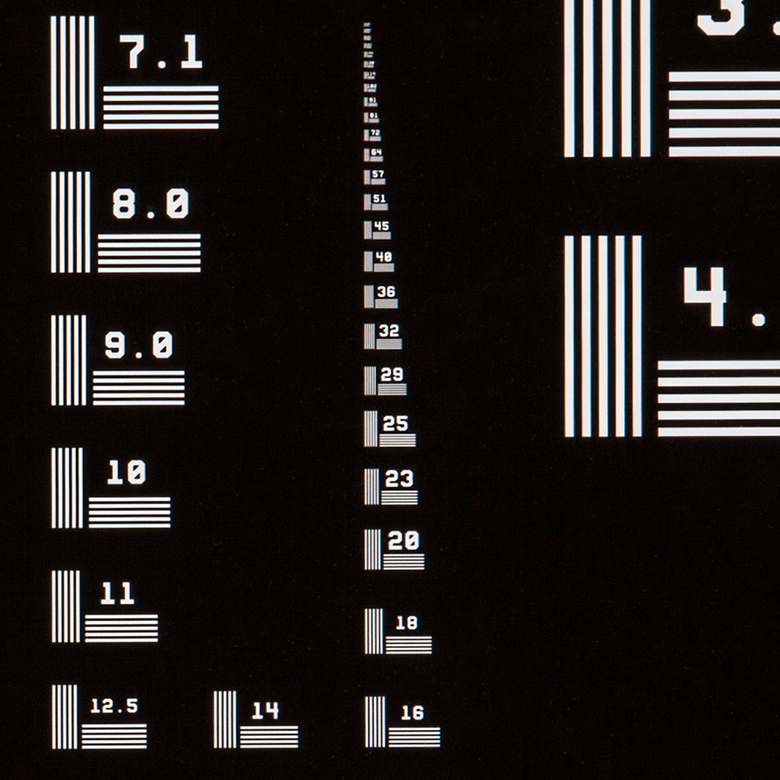
\includegraphics[width=\textwidth]{chapters/chapter_3/figures/target.jpg}
        \\
        \caption{Target}
        \label{fig:target}
    \end{subfigure}
    \hfill
    \begin{subfigure}[b]{0.55\textwidth}
        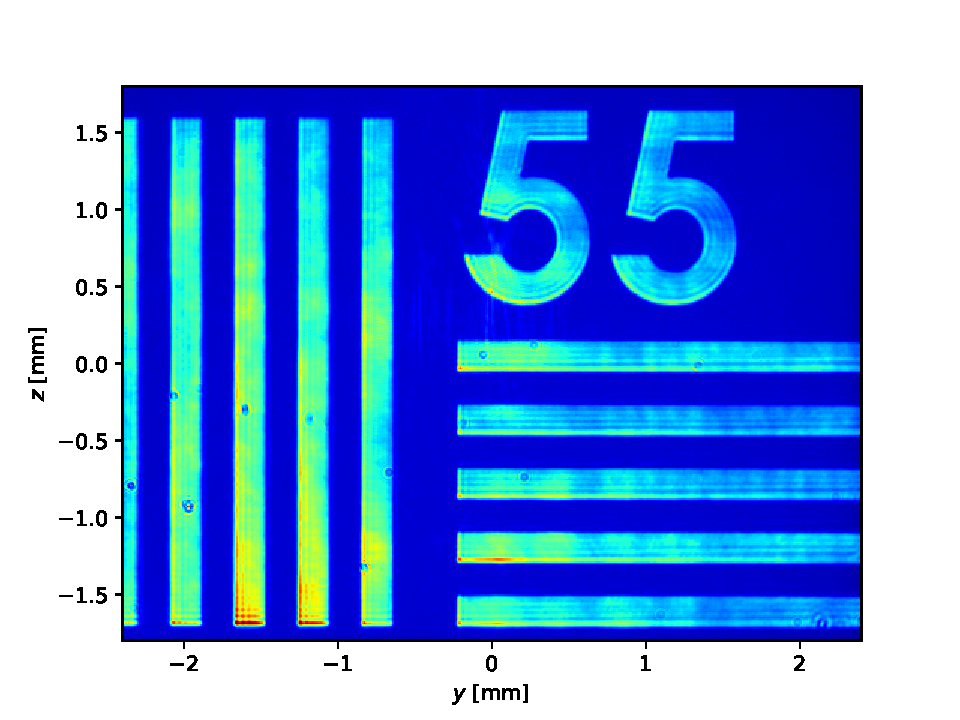
\includegraphics[width=\textwidth]{chapters/chapter_3/figures/magnified}
        \caption{Magnified image}
        \label{fig:magnified}
    \end{subfigure}
    \hfill
    \caption{Calibration of the imaging system. On the left, an example of a target similar to the one used in the experiment. On the right, the magnified image of a portion of the target. The number 55 means that the target has 55 lines / \si{mm}.}
\end{figure}

\subsection{Test with the $0 - \pi$ phase plate}
\begin{figure}
    \centering
    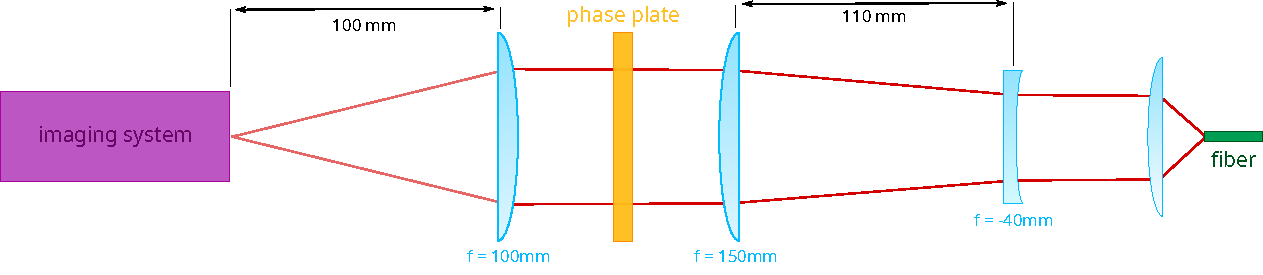
\includegraphics[width=0.9\textwidth]{chapters/chapter_3/figures/0pi_setup.pdf}
    \caption{Setup for the test of the $0-\pi$ phase plate. The beam coming from the fiber is collimated by a single lens, then expanded by two cylindrical lenses and sent to the phase plate. After the phase plate, an $f=\SI{100}{mm}$ lens is placed and the result is imagined at the focal plane of the last lens. The two cylindrical lenses and the phase plate are mounted on a rotation mount.}
    \label{fig:0pi_setup}
\end{figure}

Before characterizing the top hat phase plate, the setup was tested on the $0-\pi$ phase plate similar to the one currently used in the experiment. The laser beam coming from a fiber was collimated with a lens. Then, the beam was expanded in the $z$ direction by a telescope made of two cylindrical lenses ($f=-40/150$~mm). The expansion of the beam helped achieve higher trapping frequencies. The beam was then directed to the phase plate and to a $f=\SI{100}{mm}$ lens. The two cylindrical lenses and the phase plate were mounted on a rotation mount, to allow the alignment of their axis. The result was imaged by the imaging system at the focal plane of the last lens. The focus was adjusted by moving the imaging system along the $x$ direction. A sketch of this setup is shown in \cref{fig:0pi_setup}.

\begin{figure}
    \centering
    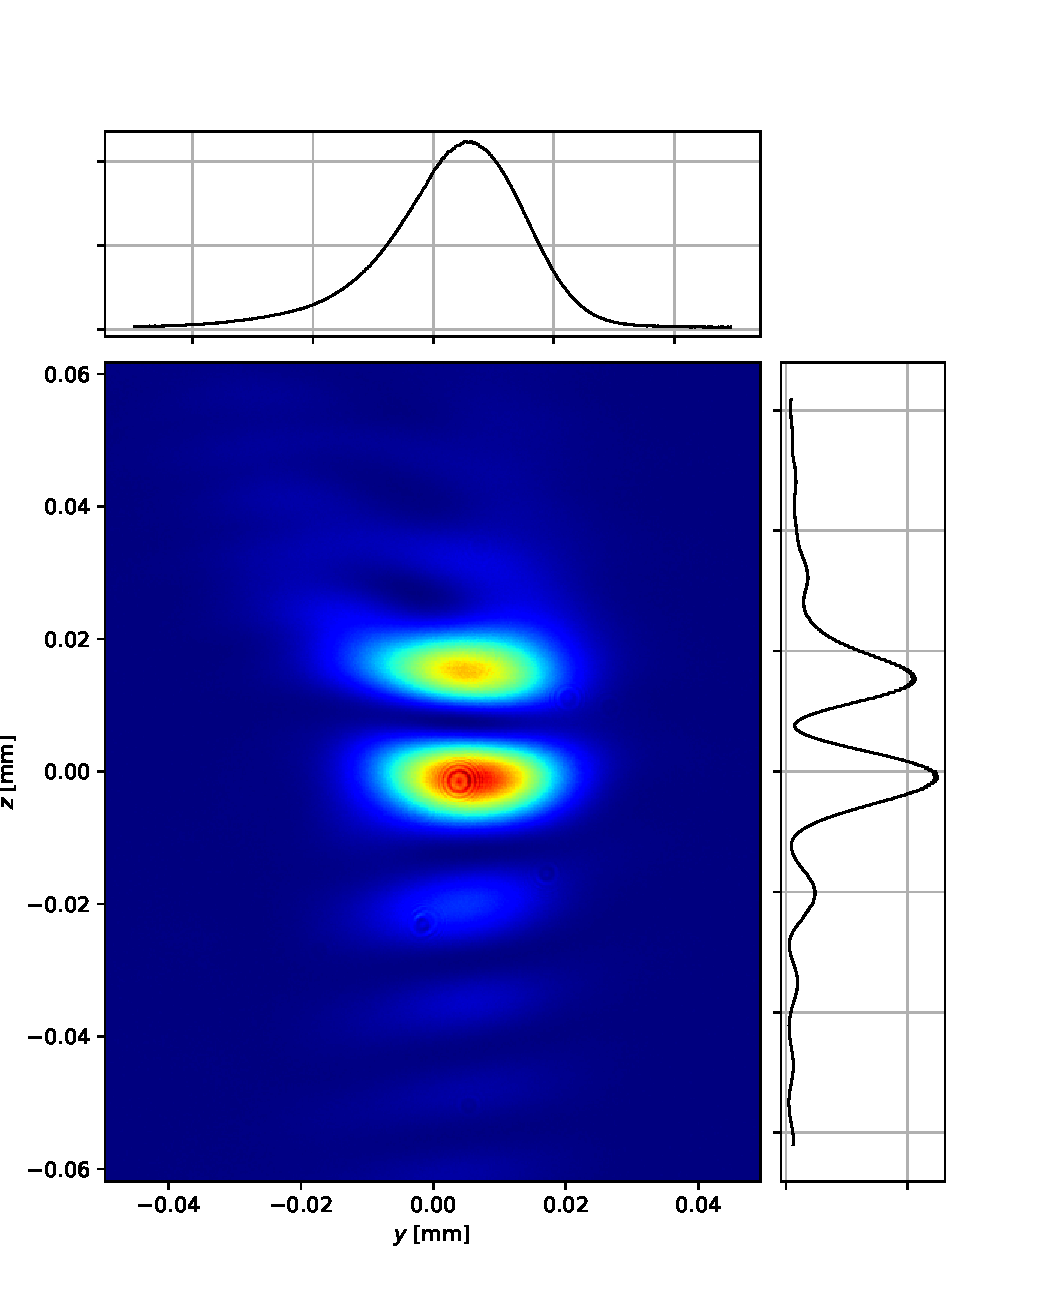
\includegraphics[width=0.5\textwidth]{chapters/chapter_3/figures/0pi_image.pdf}
    \caption{Intensity distribution after the $0-\pi$ phase plate. The size shown on the axis is the real size of the beam. The plots on the right and on top of the image show the integrated sum of the intensity along the respective axes.}
    \label{fig:0pi_image}
\end{figure}


In order to get good results, it was important that the two cylindrical lenses and the phase plate axes were aligned. To align them, the beam was observed at short and long distances. Acting on the first lens, the beam was rotated in such a way that, when observed at a short distance, its axis was vertical. The same alignment was then performed acting on the second cylindrical lens and looking at the beam at a longer distance. The procedure was repeated, \enquote{walking} the beam, until the two lenses were aligned. The collimation of the beam was ensured by using a shear plate. Finally, the phase plate was aligned rotating its axis in such a way that it was parallel to the beam axis.

The final result is shown in \cref{fig:0pi_image}. The result resembles the expected $\text{TEM}_{01}$ mode shown in \cref{fig:tem10}, but it is clear that it could be optimized, making it more symmetric. In particular, the alignment of the whole setup could have been improved.  However, since the characterization of the $0-\pi$ phase plate was not the goal of the project, the alignment was not refined. Nonetheless, this test was useful to gain familiarity with how phase plates work and with the optics involved in the setup.

\subsection{Shaping the input beam}
It had already been reported in Schmidt's work that the most crucial parameter to make the phase plate work is the beam diameter \cite{schmidt2021}. The phase plate was ordered for a diameter of \SI{6}{mm}, so this is the first thing we tried to achieve.

\subsubsection{Single collimating lens + x2 telescope}
Initially we tried to collimate the beam coming from the fiber with a single lens, chosen to produce a \SI{3}{mm} beam. Expanding the beam with a $\times 2$ telescope, composed of a $f=\SI{50}{mm}$ and a $f=\SI{100}{mm}$ achromatic lenses placed \SI{150}{mm} apart, we expected a final beam with a diameter of \SI{6}{mm}. We first tried to collimate the beam with a \SI{15.3}{mm} C260-TME-A lens (\cref{fig:beam_f15.3}), but the beam was smaller than \SI{3}{mm}. Then we tried two \SI{18.4}{mm} lens (\cref{fig:beam_f18.4_small,fig:beam_f18.4_large}). The diameter of the former (C280-TMD-A) was too small ($\approx \SI{3}{mm}$, close to the beam diameter), and produced a beam with many aberrations; the latter, with a larger diameter, seemed to solve the problem. The beam was then magnified by the telescope, resulting in the picture shown in \cref{fig:beam_f18.4x2}.

\begin{figure}[t!]
    \begin{subfigure}{0.5\textwidth}
        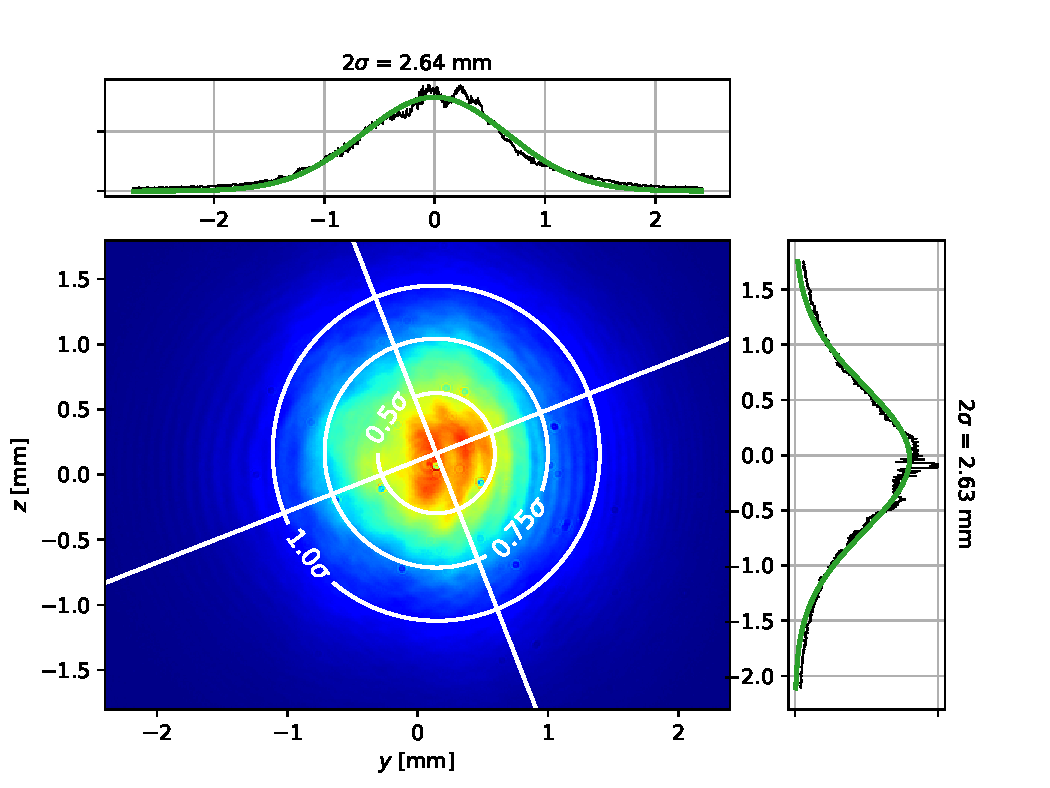
\includegraphics[width=\textwidth]{chapters/chapter_3/figures/beam_f15.3.pdf}
        \caption{f = \SI{15.3}{mm}}
        \label{fig:beam_f15.3}
    \end{subfigure}
    \begin{subfigure}{0.5\textwidth}
        \centering
        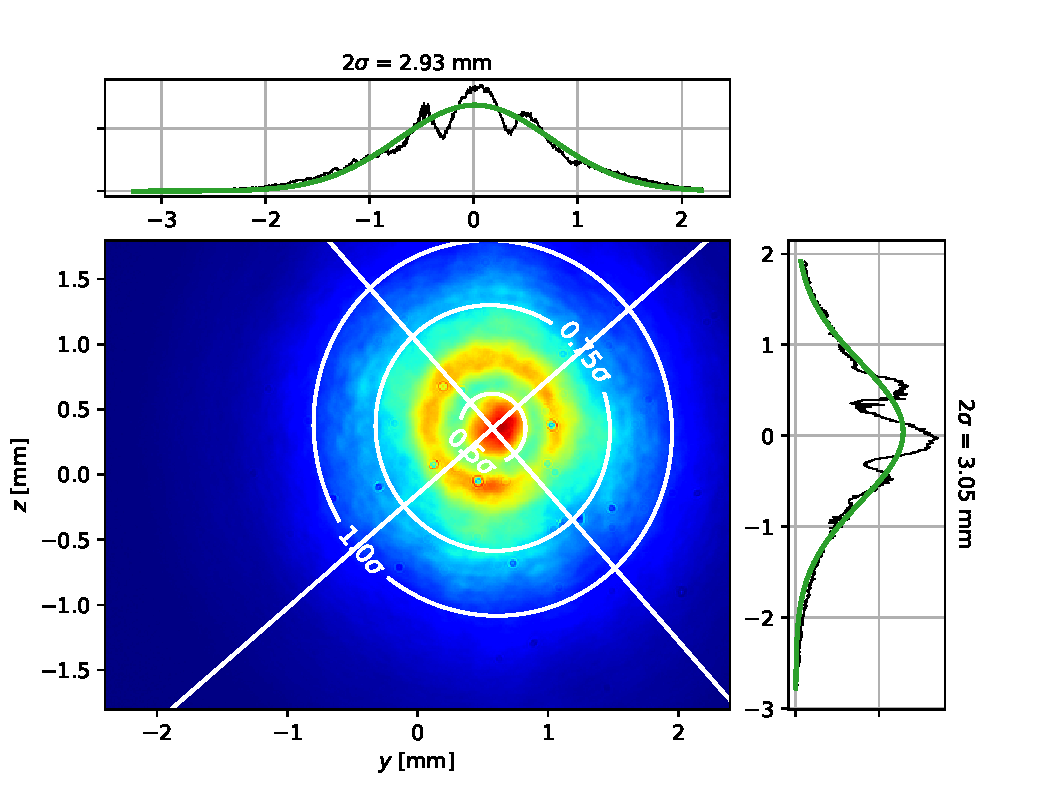
\includegraphics[width=\textwidth]{chapters/chapter_3/figures/beam_f18.4_small.pdf}
        \caption{f = \SI{18.4}{mm}, small diameter}
        \label{fig:beam_f18.4_small}
    \end{subfigure}
    \begin{subfigure}{0.5\textwidth}
        \centering
        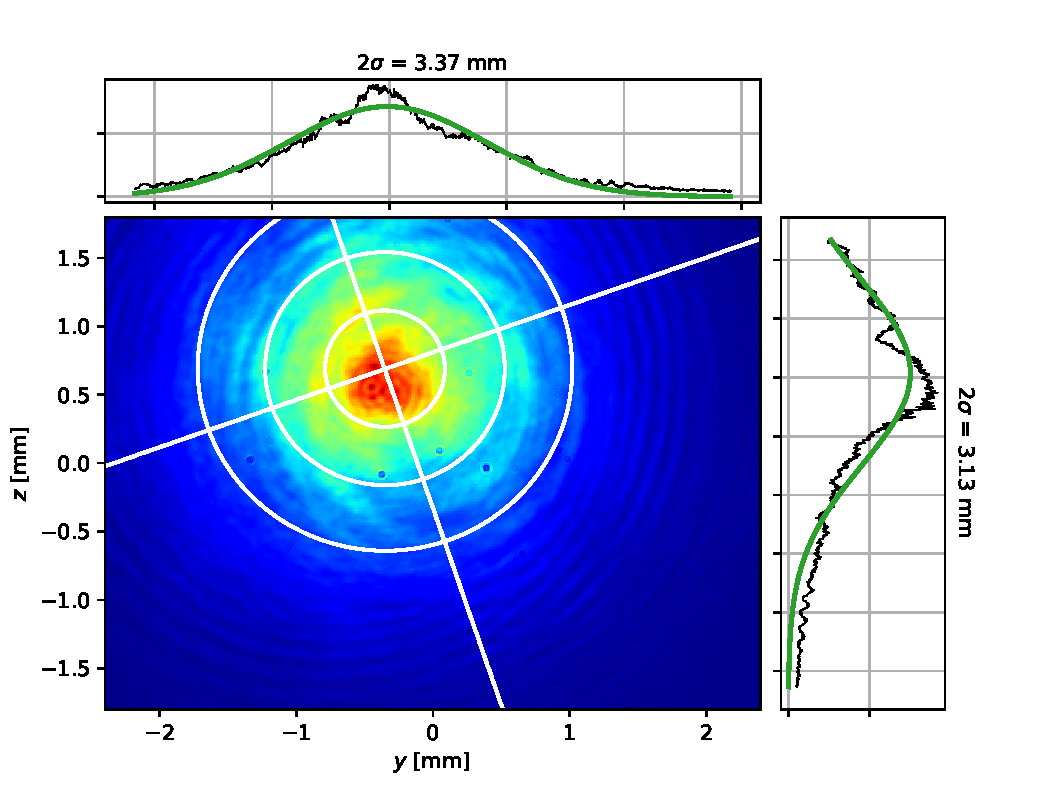
\includegraphics[width=\textwidth]{chapters/chapter_3/figures/beam_f18.4_large.pdf}
        \caption{f = \SI{18.4}{mm}, large diameter}
        \label{fig:beam_f18.4_large}
    \end{subfigure}
    \begin{subfigure}{0.5\textwidth}
        \centering
        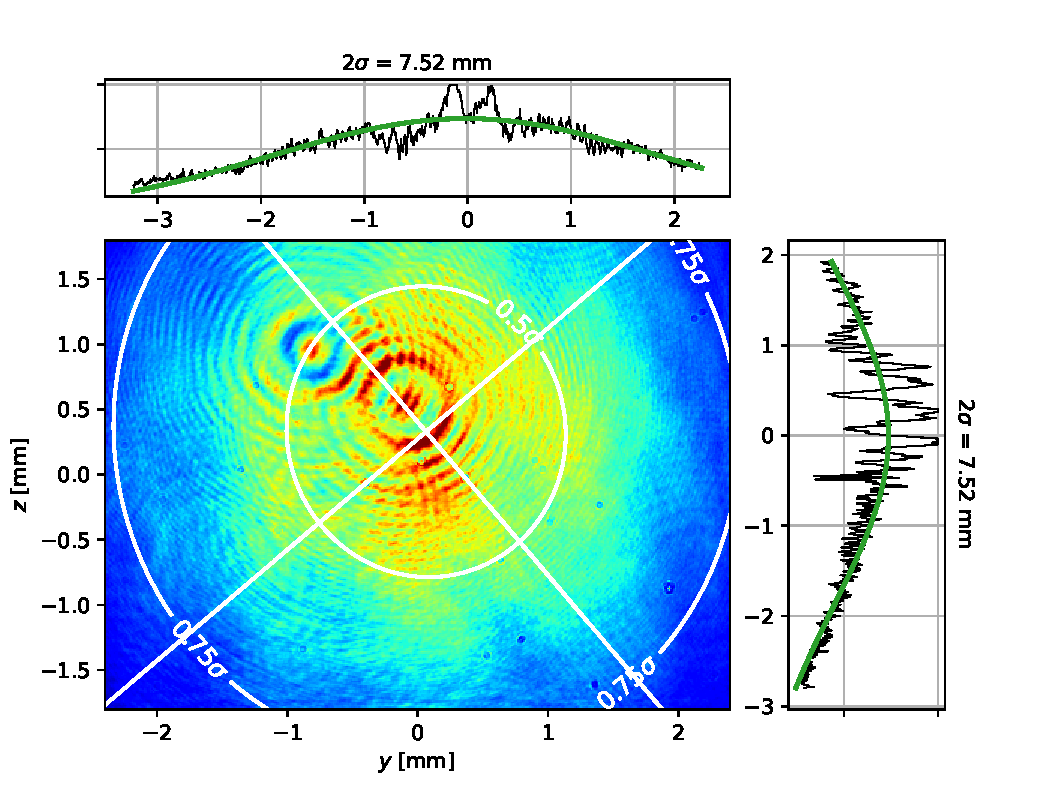
\includegraphics[width=\textwidth]{chapters/chapter_3/figures/beam_f18.4x2.pdf}
        \caption{f = \SI{18.4}{mm}, x2 telescope}
        \label{fig:beam_f18.4x2}
    \end{subfigure}
    \caption{Beam collimation with a single lens. The focal length of each lens is indicated below the respective figure. In figure (b) and (c) the lenses have the same focal length but different diameter. In figure (d) the beam is magnified with a $\times 2$ telescope.}
\end{figure}

Given the bad result, we decided to try with a different configuration.

\begin{figure}[p]
    \begin{subfigure}{0.5\textwidth}
        \centering
        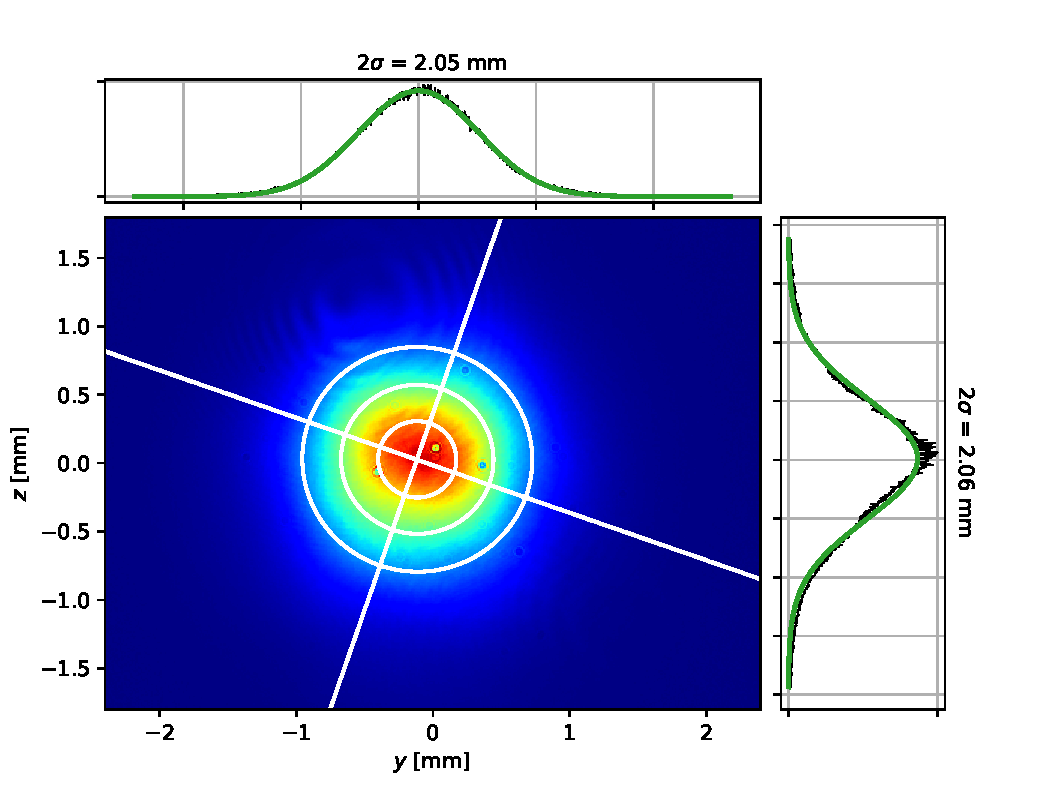
\includegraphics[width=\textwidth]{chapters/chapter_3/figures/beam_f12.pdf}
        \caption{f = \SI{12}{mm}}
        \label{fig:beam_f12}
    \end{subfigure}
    \begin{subfigure}{0.5\textwidth}
        \centering
        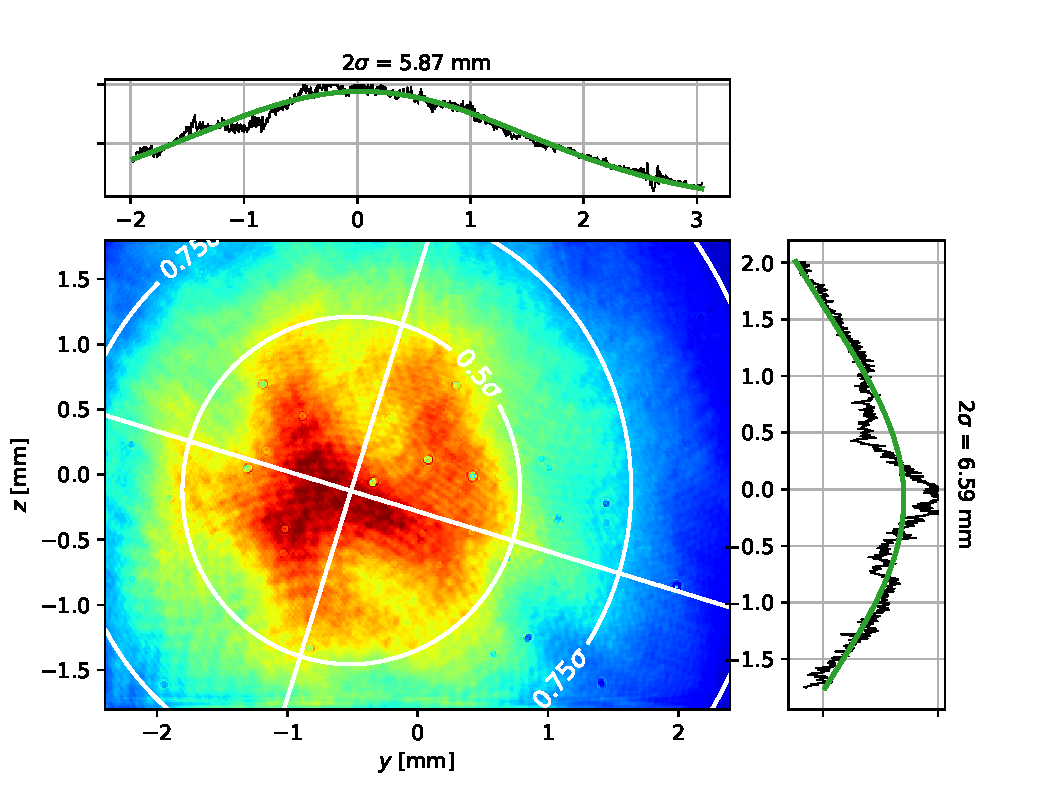
\includegraphics[width=\textwidth]{chapters/chapter_3/figures/beam_f12x3.pdf}
        \caption{f = \SI{12}{mm}, $\times3$ telescope}
        \label{fig:beam_f12x3}
    \end{subfigure}
    \\
    \hfill
    \begin{subfigure}{\textwidth}
        \centering
        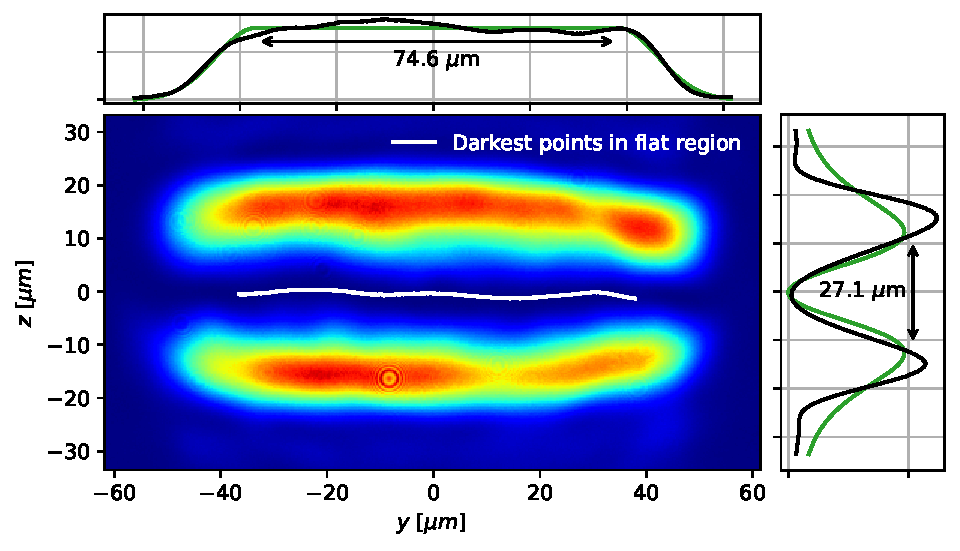
\includegraphics[width=0.5\textwidth]{chapters/chapter_3/figures/tophat_f12x3.pdf}
        \caption{Top hat distribution}
        \label{fig:tophat_f12x3}
    \end{subfigure}
    \hfill
    \caption{Beam collimation with a \SI{12}{mm} Schäfter-Kirchhoff collimator, magnified with a $\times3$ telescope ((a) and (b)).  The meaning of the fits in (c) are explained \cref{sec:characterization_methods}.}
    \label{fig:f12mm}
\end{figure}

\subsubsection{Schäfter-Kirchhoff collimator + $\times 3$ telescope}
In the second configuration, we collimated the beam with a Schäfter-Kirchhoff collimator (60FC-4-M12-10, $f=\SI{12}{mm}$). The collimator was expected to produce a beam with a diameter of $\approx \SI{2}{mm}$, which therefore required a $\times3$ telescope. The telescope was assembled using a \SI{-50}{mm} lens and a \SI{150}{mm} lens. Both lenses were achromatic lenses. The use of a concave and a convex lens, beside reducing aberrations, allowed to keep the setup more compact. The beams before and after the telescope are shown in \cref{fig:beam_f12,fig:beam_f12x3}.
In \cref{fig:tophat_f12x3} it is also shown the profile of the beam after being shaped by the phase plate in combination with a \SI{100}{mm} lens. It is clear that, despite the general features of the top hat distribution being present, the intensity distribution is very different from the expected one. In particular the top and bottom light sheets seem to be curved around the centre.

\subsubsection{Single collimating lens}
To improve the previous result, we tried to reduce the aberrations using a single achromatic lens to collimate the beam directly to the desired size. In particular, we tried two different lenses: TRH254-040-A-ML ($f=\SI{40}{mm}$) and MG 01LAO785 ($f=\SI{37.5}{mm}$). The results are shown in \cref{fig:beam_single_lens}. Also with this configuration, the result was disappointing, since the beam deviated a lot from the expected Gaussian profile.

\begin{figure}[p]
    \begin{subfigure}{0.5\textwidth}
        \centering
        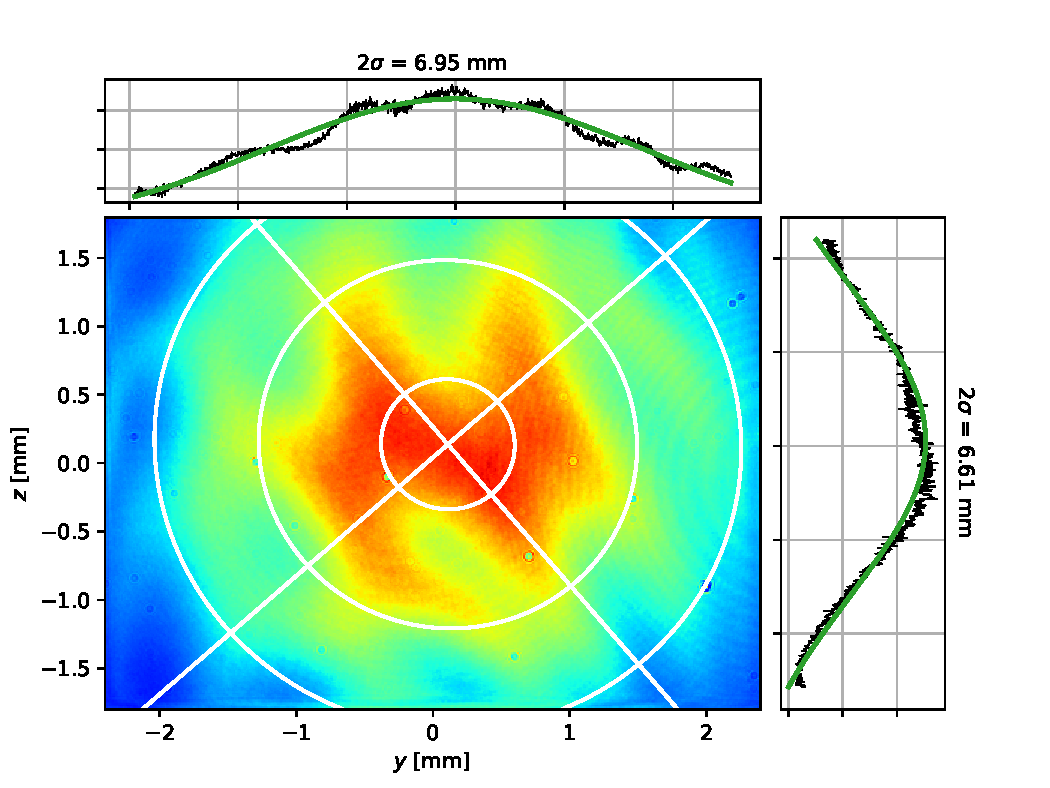
\includegraphics[width=\textwidth]{chapters/chapter_3/figures/beam_f40.pdf}
        \caption{f = \SI{40}{mm}}
        \label{fig:beam_f40}
    \end{subfigure}
    \begin{subfigure}{0.5\textwidth}
        \centering
        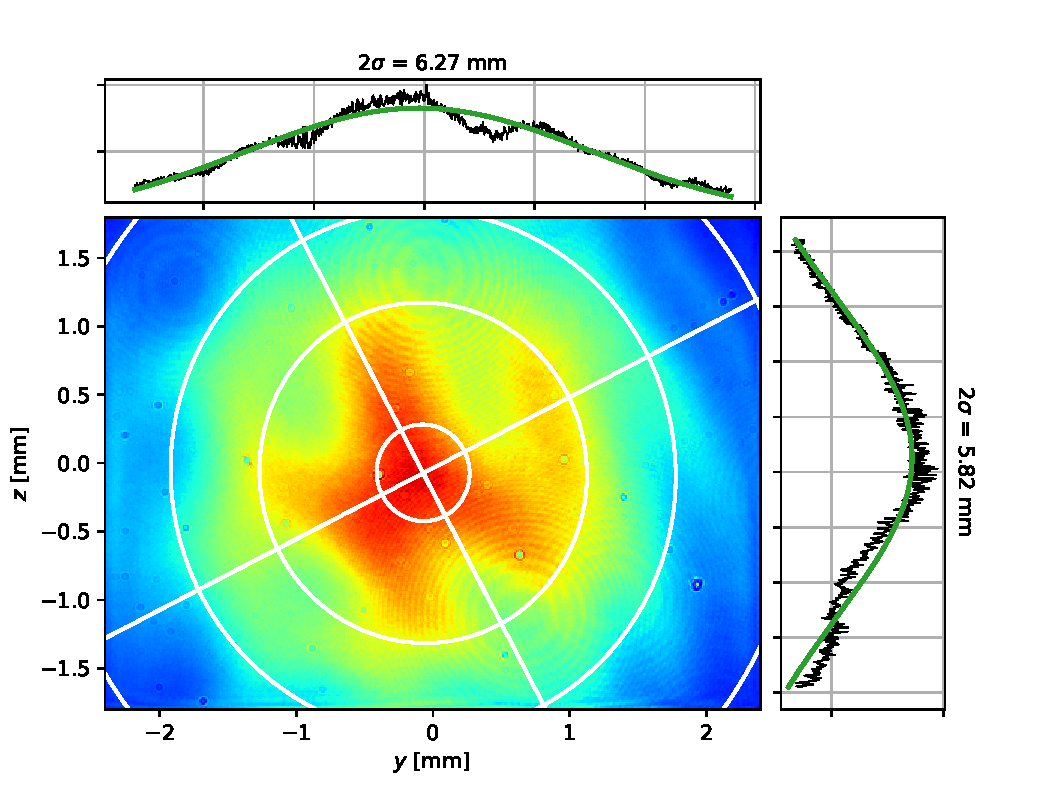
\includegraphics[width=\textwidth]{chapters/chapter_3/figures/beam_f37.pdf}
        \caption{f = \SI{37.5}{mm}}
        \label{fig:beam_f37.5}
    \end{subfigure}
    \caption{Beam collimation with a single lens.}
    \label{fig:beam_single_lens}
\end{figure}

\subsubsection{Schäfter-Kirchhoff collimator}
Since we were not able to achieve good results only with the optics we had in the lab, we decided to order a collimator with the desired features. In particular, we ordered a Schäfter-Kirchhoff 60FC-L-4-M35-26 collimator ($f = \SI{35}{mm}$), specifically designed to collimate large beams. In \cref{fig:collimator} we show the beam and the result after shaping it with the phase plate and a \SI{100}{mm} lens. Surprisingly, the result was even worse than the previous ones. Placing the phase plate in the far field with respect to the collimator did not change the result appreciably. Also trying to reduce the aberrations by adding a 1:1 telescope with a pinhole in between did not have any noticeable effects.

\begin{figure}
    \begin{subfigure}{0.5\textwidth}
        \centering
        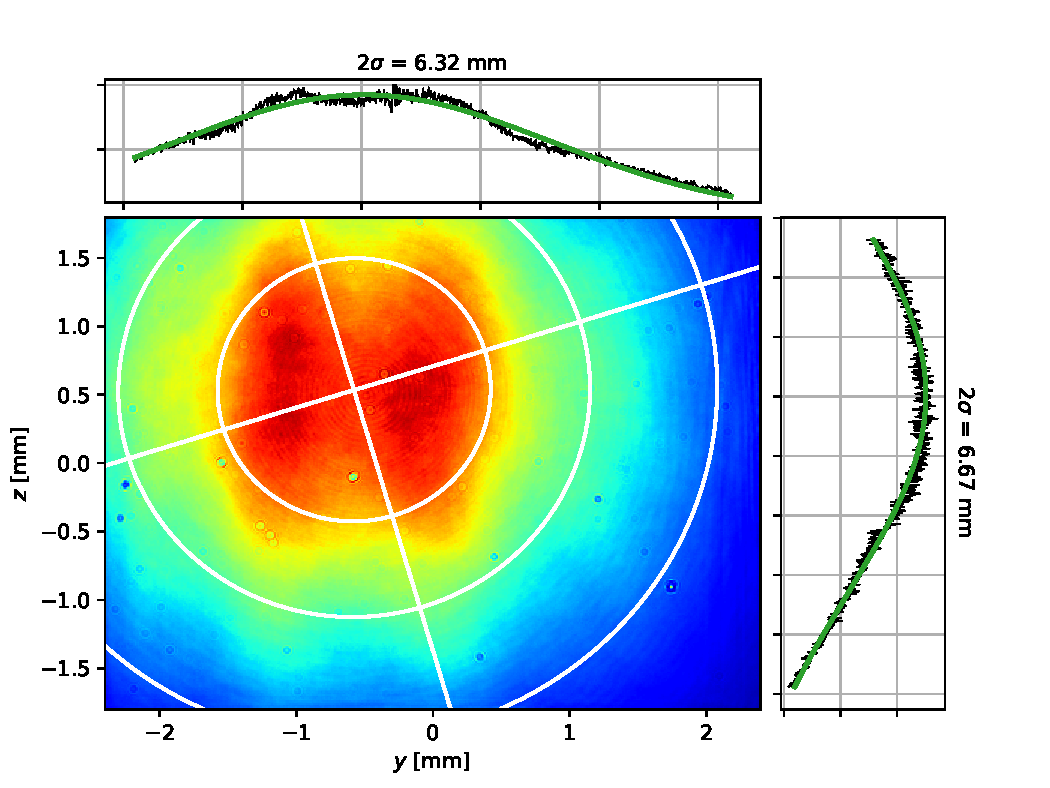
\includegraphics[width=\textwidth]{chapters/chapter_3/figures/beam_f35.pdf}
        \caption{Beam}
        \label{fig:beam_f35}
    \end{subfigure}
    \begin{subfigure}{0.5\textwidth}
        \centering
        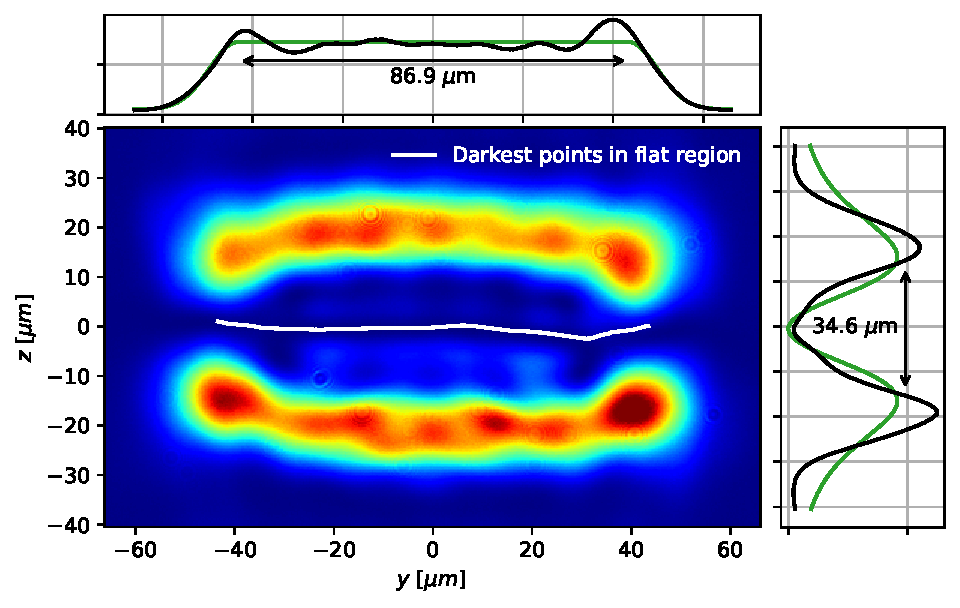
\includegraphics[width=\textwidth]{chapters/chapter_3/figures/tophat_f35.pdf}
        \caption{Top hat}
        \label{fig:tophat_f35}
    \end{subfigure}
    \caption{Beam collimation with a Schäfter-Kirchhoff \SI{35}{mm} collimator. The first image shows the beam after the collimator. The second image shows the top hat distribution generated by the phase plate together with a \SI{100}{mm} lens. The meaning of the fits in (b) are explained \cref{sec:characterization_methods}.}
    \label{fig:collimator}
\end{figure}

\subsubsection{Schäfter-Kirchhoff collimator + $\times 3$ telescope with varying beam size}

Since even in the (theoretically) best configuration, i.e. using a collimator designed to produce a beam of the desired size, the result was far from optimal, we thought that the problem may have resided in the beam size itself. Therefore, we decided to investigate the influence of the beam diameter on the result more systematically. To do so, we went back to the configuration with the Schäfter-Kirchhoff \SI{12}{mm} collimator and the $\times3$ telescope, with which we had obtained the best result so far (\cref{fig:f12mm}).
To vary the size of the beam, instead of using the collimator in its usual way, we manually adjusted it to produce a non-collimated beam. A diverging (converging) beam directed to the telescope produced a final beam larger (smaller) than a collimated one. Moving the second lens of the telescope back and forth, it was possible to re-collimate the beam. In this way, we could vary the size of the beam keeping it collimated at the phase plate  position. A sketch of this configuration is shown in \cref{fig:adjustable_setup}

\begin{figure}
    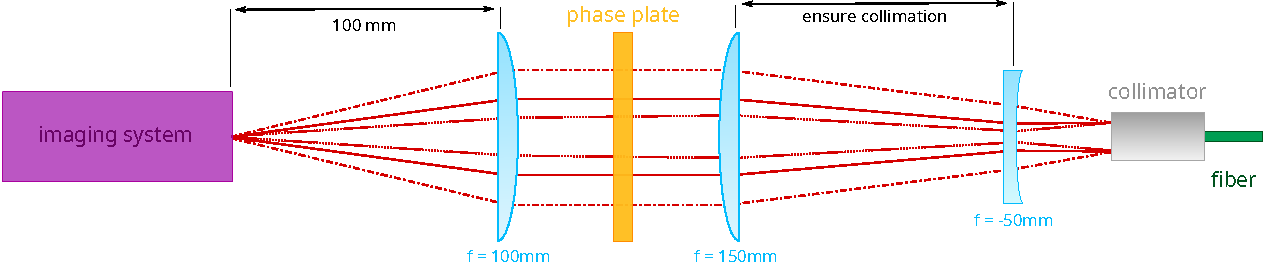
\includegraphics[width=\textwidth]{chapters/chapter_3/figures/adjfoc_setup.pdf}
    \caption{Setup for the test of the top hat phase plate for various beam sizes. The beam coming from the fiber is (not perfectly) collimated by a Schäfter-Kirchhoff collimator, then expanded and collimated by two lenses and sent to the phase plate. After the phase plate, an $f=\SI{100}{mm}$ lens is placed and the result is imaged at the focal plane of the last lens.}
    \label{fig:adjustable_setup}
\end{figure}

\begin{figure}
    \begin{subfigure}{0.5\textwidth}
        \centering
        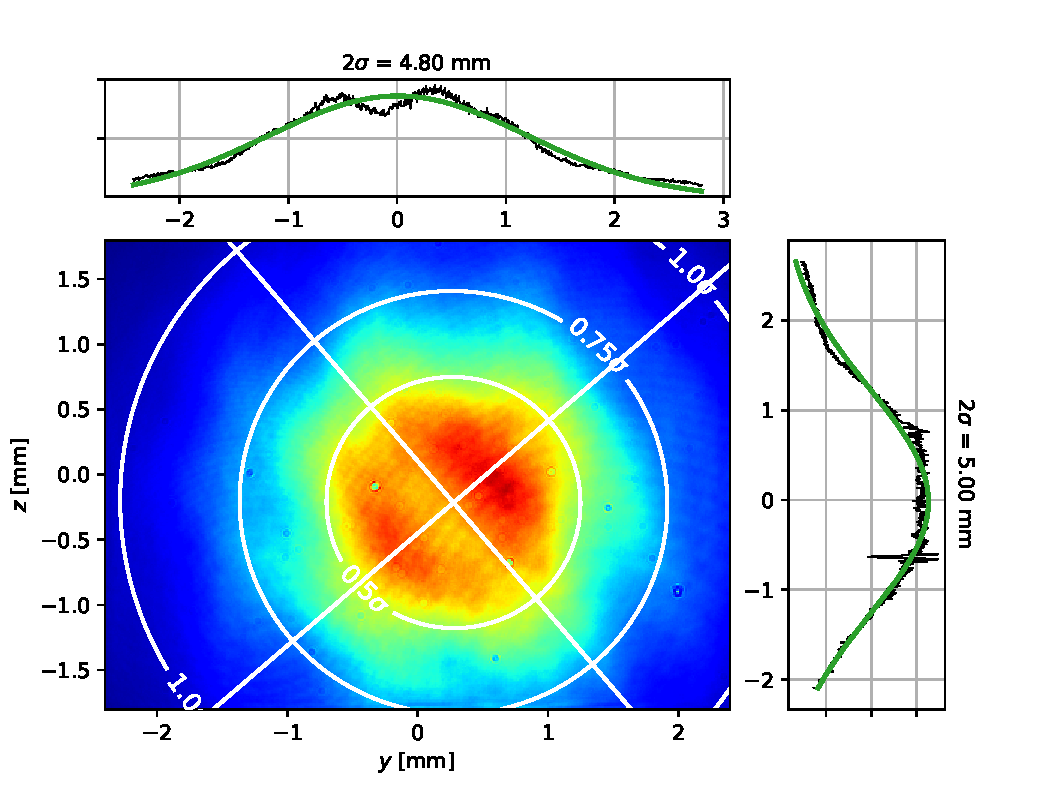
\includegraphics[height=0.75\textwidth]{chapters/chapter_3/figures/x3_sizes/beam1.pdf}
        \caption{}
        \label{fig:f12x3_small_beam}
    \end{subfigure}
    \begin{subfigure}{0.5\textwidth}
        \centering
        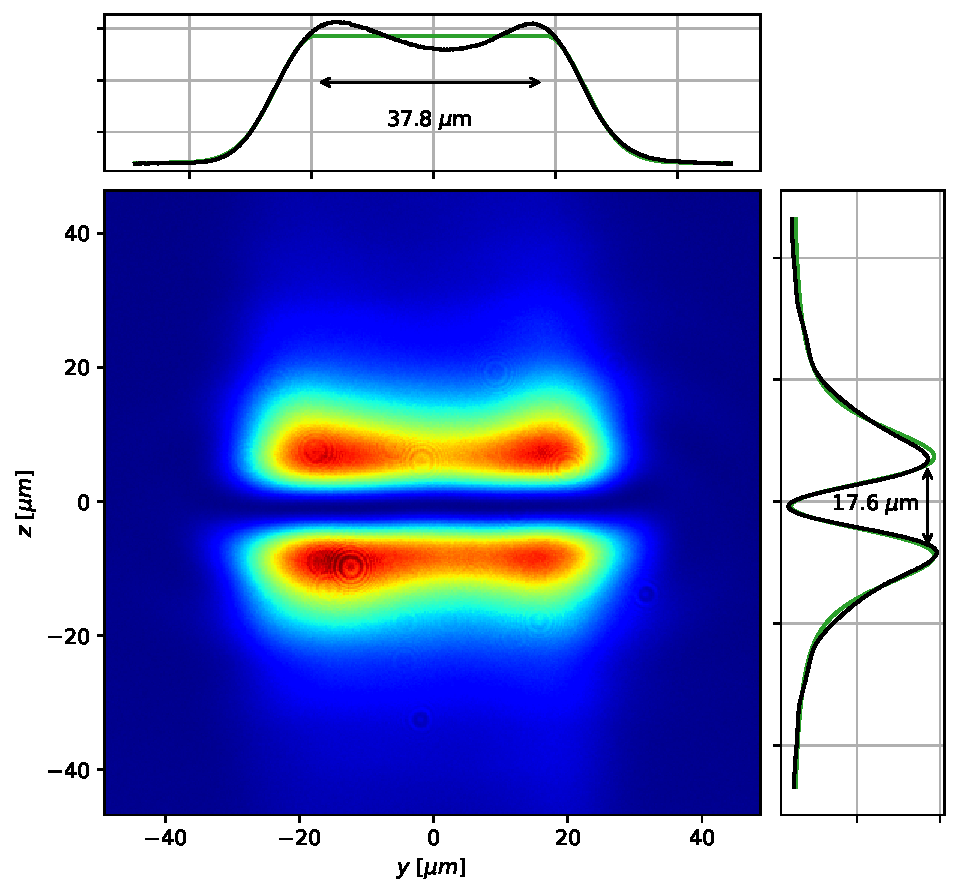
\includegraphics[height=0.7\textwidth]{chapters/chapter_3/figures/x3_sizes/tophat1.pdf}
        \caption{}
        \label{fig:f12x3_small_tophat}
    \end{subfigure}
    \begin{subfigure}{0.5\textwidth}
        \centering
        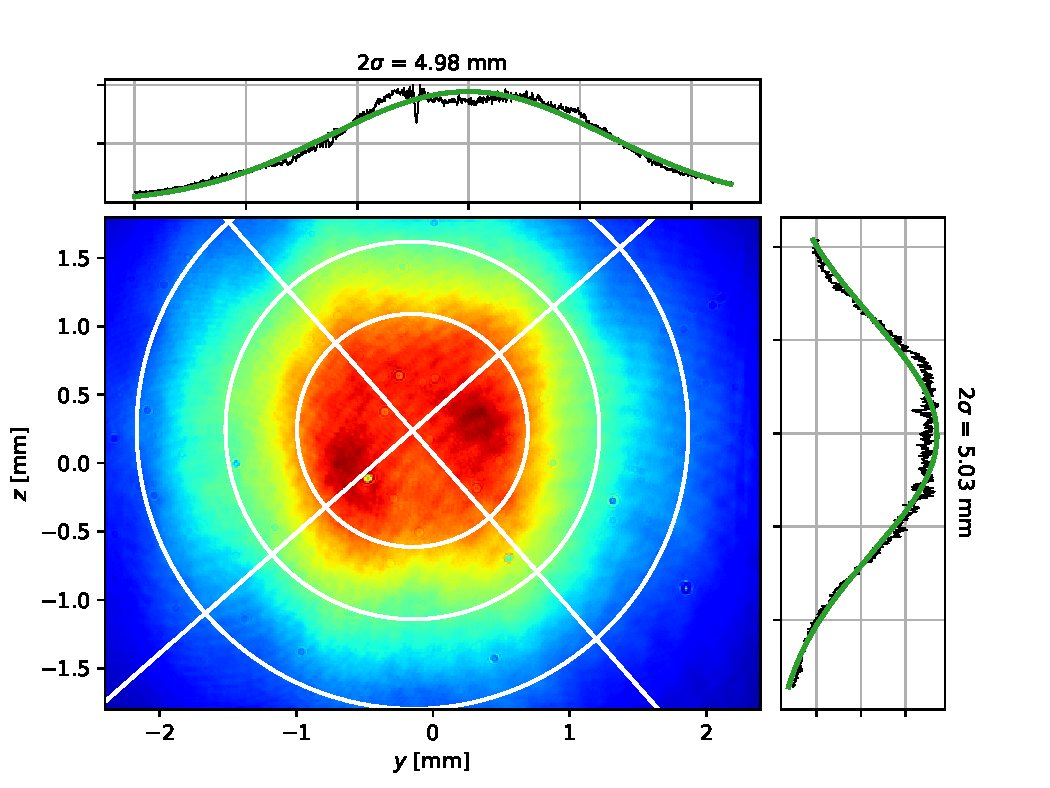
\includegraphics[height=0.75\textwidth]{chapters/chapter_3/figures/x3_sizes/beam3.pdf}
        \caption{}
        \label{fig:f12x3_medium_beam}
    \end{subfigure}
    \begin{subfigure}{0.5\textwidth}
        \centering
        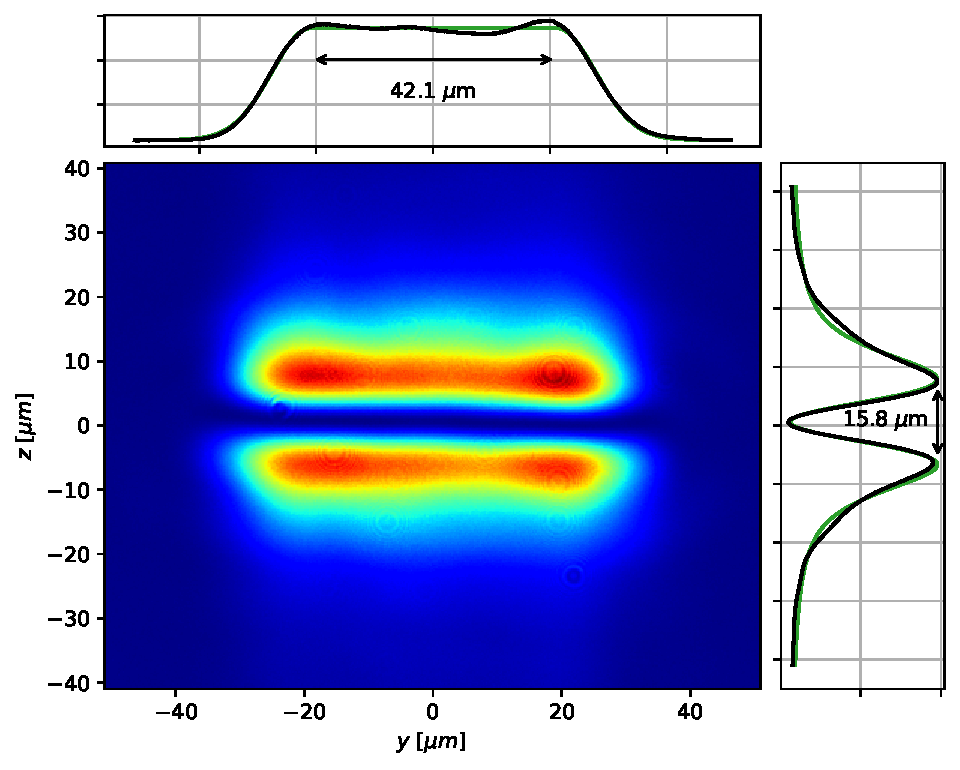
\includegraphics[height=0.7\textwidth]{chapters/chapter_3/figures/x3_sizes/tophat3.pdf}
        \caption{}
        \label{fig:f12x3_medium_tophat}
    \end{subfigure}
    \begin{subfigure}{0.5\textwidth}
        \centering
        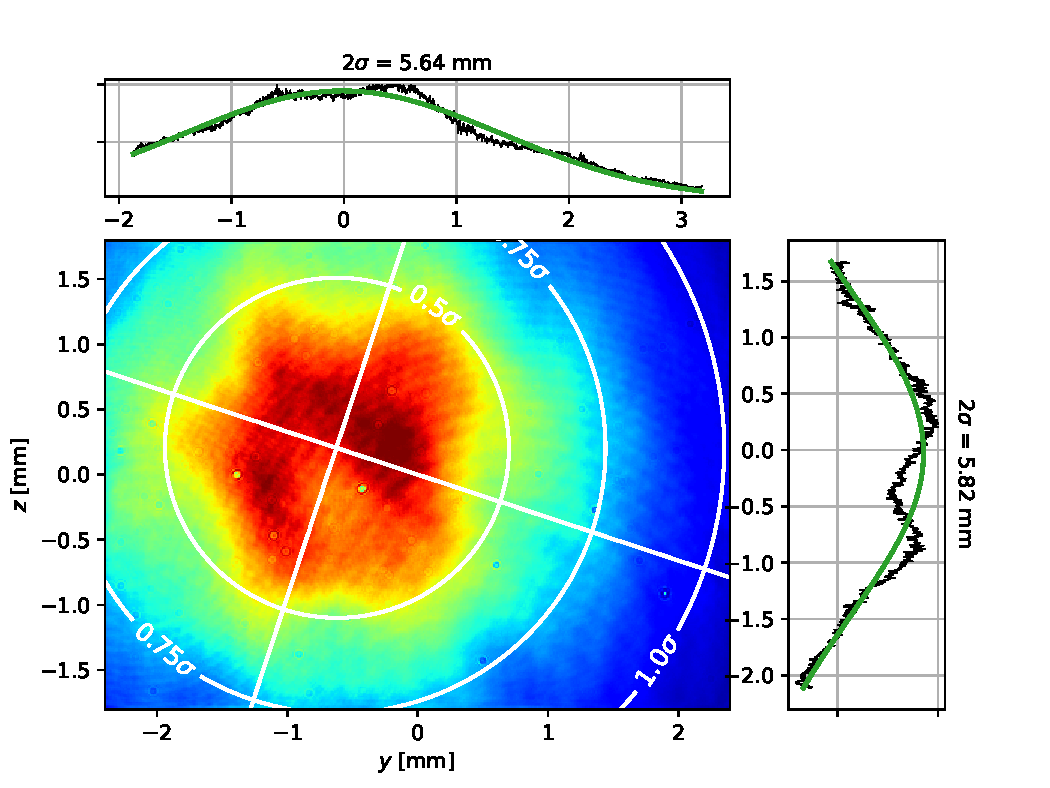
\includegraphics[height=0.75\textwidth]{chapters/chapter_3/figures/x3_sizes/beam2.pdf}
        \caption{}
        \label{fig:f12x3_large_beam}
    \end{subfigure}
    \begin{subfigure}{0.5\textwidth}
        \centering
        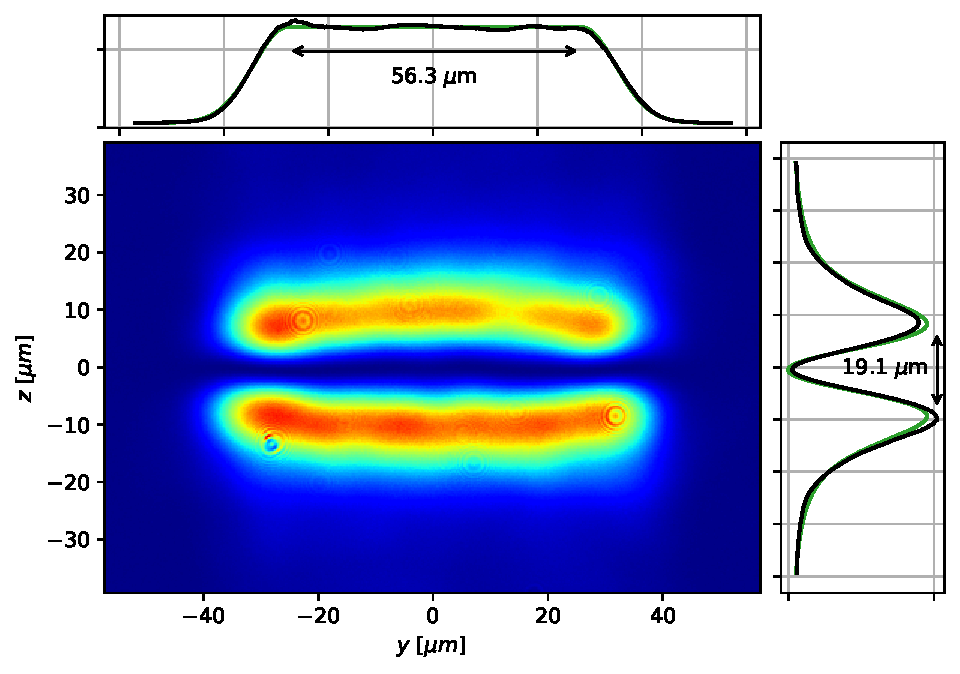
\includegraphics[height=0.7\textwidth]{chapters/chapter_3/figures/x3_sizes/tophat2.pdf}
        \caption{}
        \label{fig:f12x3_large_tophat}
    \end{subfigure}
    \caption{Beam and top hat distribution for different beam sizes. Every row shows a beam on the left and its respective top hat distribution on the right. The results were obtained
        with the \SI{12}{mm} collimator and together with the $\times3$ telescope. The meaning of the fits on the top hat images are explained \cref{sec:characterization_methods}.}
    \label{fig:f12x3_sizes}
\end{figure}

The results, for three different sizes of the beam, are collected in \cref{fig:f12x3_sizes}. From the figures, it is clear that the dimension of the beam has a big influence on the result. Even changes of fractions of a millimetre produce great differences in the final result. In particular, it is interesting to observe that for large beams we recognize the behaviour observed in all the previous configurations, i.e. a curvature of the two light sheets around the centre. On the other hand, small beams produce an uneven intensity distribution along the $y$ axis, with peaks at the border of the flat region. A good compromise seems to be found for a beam of $\approx \SI{5}{mm}$. This explains the bad results obtained before, since we were using much larger beams, even if the size was similar to the specifications given by the manufacturer.

\section{Characterization}
\label{sec:characterization}
Having found a good beam size which we could aim for, we decided to assemble a telescope that would give us approximately the desired size, and use it to fully characterize the phase plate. For the characterization of the phase plate we decided to keep using the Schäfter-Kirchhoff \SI{12}{mm} collimator, but instead of expanding the beam with a $\times3$ telescope, we used a $\times2.4$ one. With this setup, we expected a beam with a diameter of $\approx \SI{4.8}{mm}$, size for which we had previously found a good result. The telescope was built with a \SI{-50}{mm} and a \SI{120}{mm} achromatic lenses.

For a complete characterization of the phase plate, it was necessary to analyse its behaviour for different beam sizes and different distances from the focus. It was important to look at the light sheet at different distances from the focus because, despite the focal point being in principle well-defined, finding it was non-trivial. Moreover, we did not know if for our goals a non-perfectly focused beam may have been better than a focused one.

\subsection{Methods}
\label{sec:characterization_methods}
Before presenting the results, we offer a brief overview of the methods used to characterize the phase plate. The goal is to define a couple of quantities that can tell us how \enquote{good} results are compared to each other, allowing us to find the best possible configuration.

\subsubsection{Beam characterization}
Before diving into the different parameters that were defined to characterize the quality of the light sheet, we briefly mention how the beam itself was characterized. After ensuring the collimation of the beam through the use of a shear plate, a picture of it was taken with a camera. The resulting image was fitted to a 2D Gaussian of the form
\begin{equation}
    G(\mathbf{x}) = G_0 + A \exp[-(\mathbf{x}-\mathbf{x_0})^T \bar{\Sigma} (\mathbf{x}-\mathbf{x_0})]
\end{equation}
where $\mathbf{x} = (x,y)$ and $\mathbf{x_0} = (x_0,y_0)$ is the centre of the Gaussian distribution. The covariance matrix
\begin{equation}
    \Sigma =
    \begin{pmatrix}
        1/2\sigma_x & 0           \\
        0           & 1/2\sigma_y
    \end{pmatrix}
\end{equation}
was rotated to $\bar{\Sigma} = R^T \Sigma R$, where $R$ is the rotation matrix. For a rotation of an angle $\theta$, this would be
\begin{equation}
    R = \begin{pmatrix*}[r]
        \cos(\theta) & -\sin(\theta) \\
        \sin(\theta) & \cos(\theta)
    \end{pmatrix*}
\end{equation}
The fit is then used to find the size of beam $\sigma_x$ and $\sigma_y$ along the two main axes.

\subsubsection{Intensity normalization}

For every combination of beam size and distance from the focus, two pictures were taken: a normal (non-satuaretd) picture and a saturated picture. The non-satuaretd picture gave us information on the intensity distribution of the whole light sheet. The saturated picture allowed us to increase the dynamic range of the image in the dark central region, increasing the precision of the measurements.
%An example of a saturated picture can be found in \cref{fig:parabola_imsat}.
To saturate the picture, we increased the exposure time. Taking note of both the exposure time of the saturated picture and of the non-satuaretd one, it was possible to \enquote{normalize} the saturated picture as
\begin{equation}
    I_\text{s}^\text{norm} = \frac{\tau_\text{ns}}{\tau_\text{s}} I_\text{s}
\end{equation}
where $\tau_\text{ns/s}$ are respectively the exposure time of the non-saturated and saturated pictures, $I_\text{s}$ the intensity measured by the camera for the saturated picture and $I_\text{s}^\text{norm}$ the normalized intensity.
For both pictures, the absolute intensity $I_\text{abs}$ was found by scaling the intensity measured by the camera $I_\text{rel}$ (already normalized for the saturated image) by a factor given by the power of the laser $P$ divided by the total power measured by the camera
\begin{equation}
    I_\text{abs}(y,z) = P\frac{I_\text{rel}(y,z)}{
        \int \differential y' \differential z' I_\text{rel}(y',z')}
\end{equation}
For all the following calculations, we assumed to have a laser with a power $P$ of $\SI{1}{W}$.

\subsubsection{Global behaviour}
The expected intensity distribution generated by the phase plate $I(y,z) = I_\text{th}(y) I_{0\pi}(z)$ is given by a top hat distribution $I_\text{th}(y)$ in the $y$ direction and by a $0-\pi$ distribution $I_{0\pi}(z)$in the $z$ direction. The top hat distribution is defined as

\begin{equation}
    I_\text{th}(y) \propto
    \begin{cases}
        \exp\left[-\left(\frac{\left|y\right|-w_F}{w_R}\right)^2\right] & \quad |y| > w_F    \\
        1                                                               & \quad |y| \leq w_F
    \end{cases}
\end{equation}
where we have defined $2w_F$ as the length of the flat region and $w_R$ as the length of the ramp-up. The $0-\pi$ distribution is given by (cf. Kircher's thesis \cite{krinner2015})
\begin{equation}
    \label{eq:erfi}
    I_{0\pi}(z) \propto  \erfi\left[\frac{z}{w_e}\right]^2 \exp\left[-2 \left(\frac{z}{w_e}\right)^2\right]
\end{equation}
where $\erfi(z) = -i\erf(iz)$ is the imaginary error function and $w_e$ an appropriate length scale. It is possible to notice that the $\erfi$ distribution multiplied by a Gaussian in \cref{eq:erfi} has two peaks distanced by $2w_e$.

Since the two variable $(y,z)$ of the intensity distribution $I(y,z)$ are theoretically independent, we can gain some first information looking at the integrated distribution of the intensity along the two axis
\begin{align}
    I_z(y) & = \int \differential z' I(y,z') \\
    I_y(z) & = \int \differential y' I(y',z)
\end{align}
and fitting the respective distributions $I_\text{th}(y)$ and $I_{0\pi}(z)$. This is what was done, for example, in \cref{fig:f12x3_medium_tophat}, for which we have found a flat region length $2w_F$ of \SI{42.1}{\micro m} and an $\erfi$ distribution with the two peaks distanced by $2w_e = \SI{19.1}{\micro m}$.

The integrated intensity $I_z(y)$ could also be used to calculate a first quantity useful to quantify the \enquote{flatness} of the top hat, the so-called peak-to-peak (P2P). The P2P is simply defined as the minimum intensity in the flat region divided by the maximum
\begin{equation}
    \label{eq:p2p}
    \text{P2P} = \min_y(I_z(y)) / \max_y(I_z(y)) \qquad |y| < w_F
\end{equation}
The closer the P2P is to one, the flatter the top hat distribution is.

\subsubsection{Local behaviour}
\begin{figure}
    \begin{subfigure}{0.45\textwidth}
        \centering
        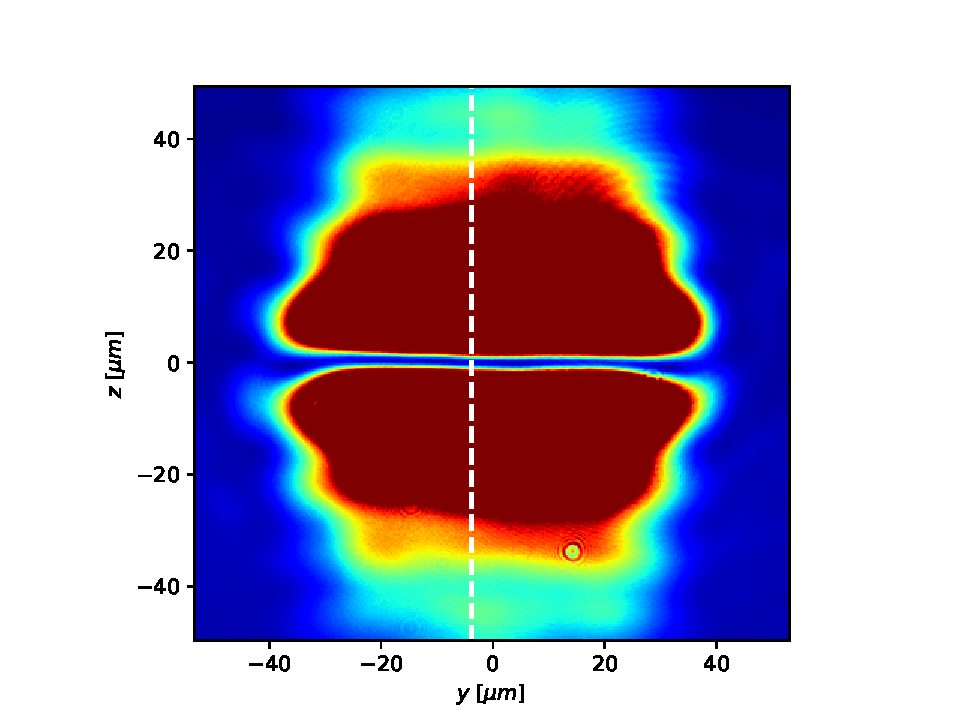
\includegraphics[height=5.25cm]{chapters/chapter_3/figures/fitquad_imsat.pdf}
        \caption{Saturated image}
        \label{fig:parabola_imsat}
    \end{subfigure}
    \begin{subfigure}{0.55\textwidth}
        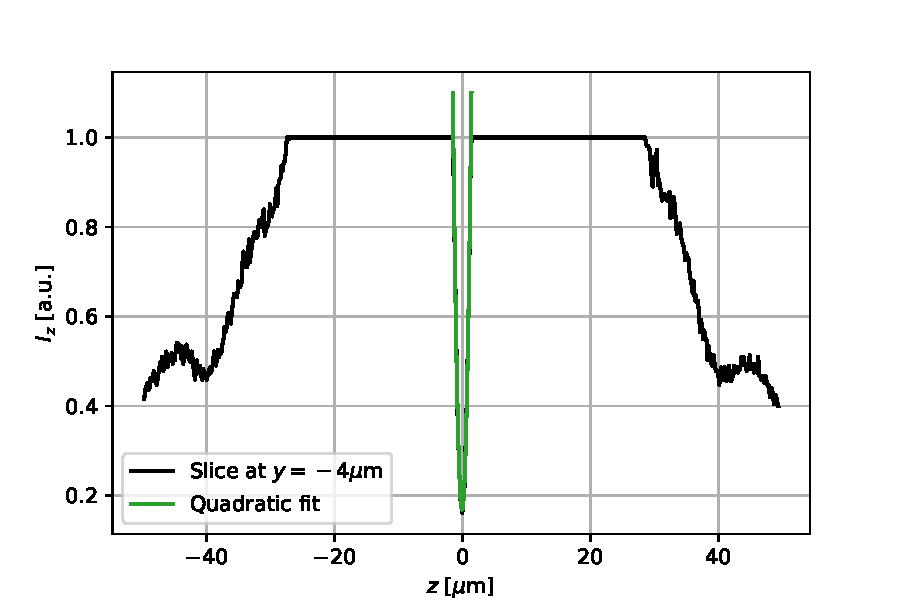
\includegraphics[height=5.25cm]{chapters/chapter_3/figures/fitquad.pdf}
        \caption{Quadratic fit}
        \label{fig:parabola_fit}
    \end{subfigure}
    \caption{Example of the quadratic fit of a slice of a saturated image. The slice is taken at $y=\SI{-4}{\micro m}$ and it has a width of a single pixel (\SI{3.75}{\micro m} on the camera and \SI{0.17}{\micro m} before magnification).}
    \label{fig:parabola}
\end{figure}

Even if the previous analysis gives us a good understanding of the global characteristics of the intensity distribution, it fails to be precise about the exact behaviour at the point we are most interested in: the central region. Since the atoms will be trapped in this region, ideally in a 2D space, they will only feel the local potential near $z=0$. It is therefore important to characterize this region with more precision.
We have already mentioned in \cref{sec:slm_specifications} that three important quantities for the characterization of the phase plate are the darkness $D(y)$, defined in \cref{eq:darkness}, the trapping frequency $\omega_z(y)$, defined in \cref{eq:trapping_frequency}, and the effective potential $U(y)$, defined in \cref{eq:effectivr_potential}. If these three quantities are evaluated for every $y$, their mean and their variation will give us information on the darkness of the region, on the strength of the trapping potential and on the uniformity of the potential.
To compute these quantities, using the saturated picture, we fitted a parabola in the $z$ direction for every $y$. We then used the fitted coefficients to compute the trapping frequency, the darkness and the effective potential. An example of a fit is shown in \cref{fig:parabola}.

\subsection{Results}

\begin{figure}
    \centering
    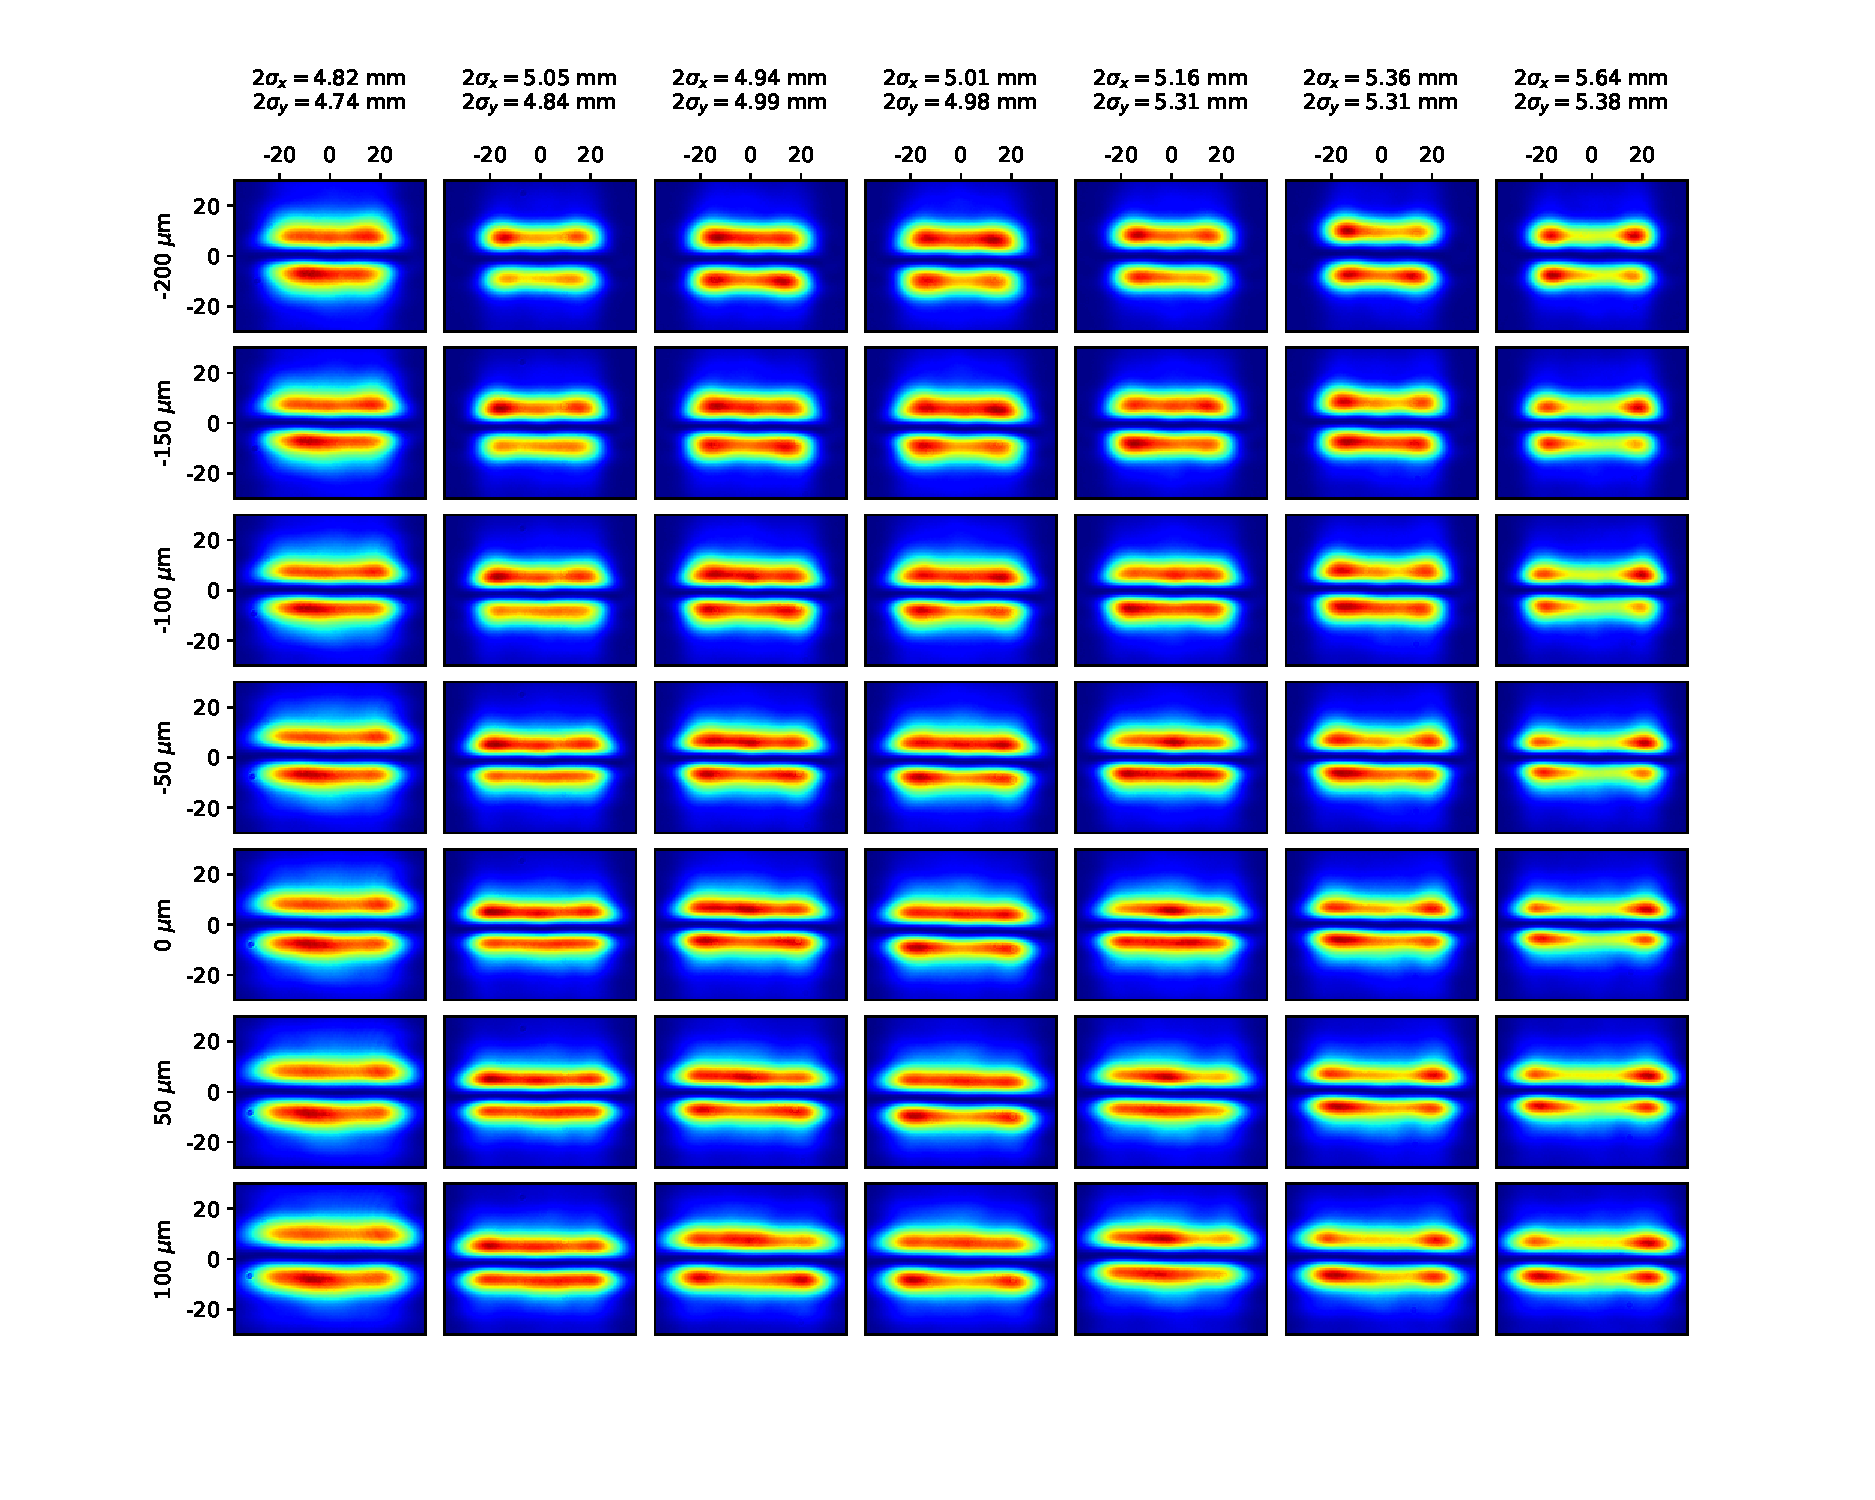
\includegraphics[width=1.3\textwidth, center]{chapters/chapter_3/figures/grid.pdf}
    \caption{Overview of the intensity distribution generated by beams of different diameters and at different focal points. The diameter of the beam along its two main axes are shown on top, while the distance from the focus is indicated on the left. The dimensions of the pictures, shown on the axes, are expressed in micrometers.}
    \label{fig:grid}
\end{figure}

Pictures were collected for different beam sizes and different distances from the focus. In total, seven beams with diameters between $\approx\SI{4.8}{mm}$ and $\approx\SI{5.5}{mm}$ were considered. For every beam size, seven pictures at seven different distances from the focus were taken. Between every picture, the imaging system was moved by \SI{50}{\micro m}. We defined the focused image as the one where the peaks found by integrating the intensity along the $y$ direction were the closest. In practice, after fitting the $0-\pi$ distribution $I_{0\pi}$ to $I_y(z)$, we chose the image for which $w_e$ was minimized (see \cref{eq:erfi} in \cref{sec:characterization_methods}). An overview of the results is shown in \cref{fig:grid}.

\subsubsection{Analysis along the focus}
We first present an analysis of the result of the phase plate modulation at different distances from the focus. Below, we discuss the case of the light sheet generated by a beam with a diameter of \SI{5}{mm} (third column in \cref{fig:grid}). An overview of the results is shown in \cref{fig:analysis_focus}.

\begin{figure}
    \begin{subfigure}{0.5\textwidth}
        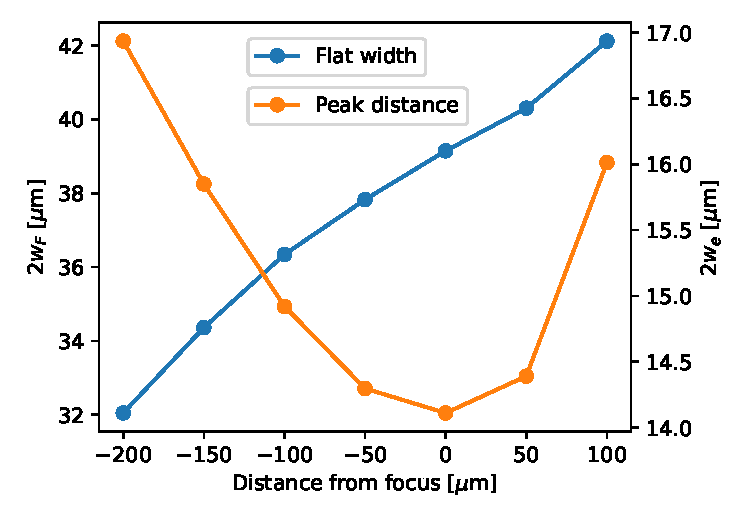
\includegraphics[width=\textwidth]{chapters/chapter_3/figures/size_focus.pdf}
        \caption{Size}
        \label{fig:focus_size}
    \end{subfigure}
    \begin{subfigure}{0.5\textwidth}
        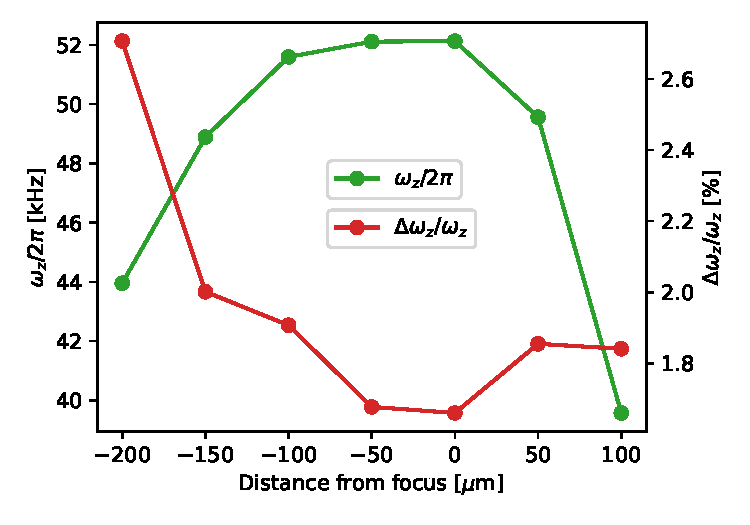
\includegraphics[width=\textwidth]{chapters/chapter_3/figures/trapp_freq_focus.pdf}
        \caption{Trapping frequency}
        \label{fig:focus_omega}
    \end{subfigure}\\

    \begin{subfigure}{0.5\textwidth}
        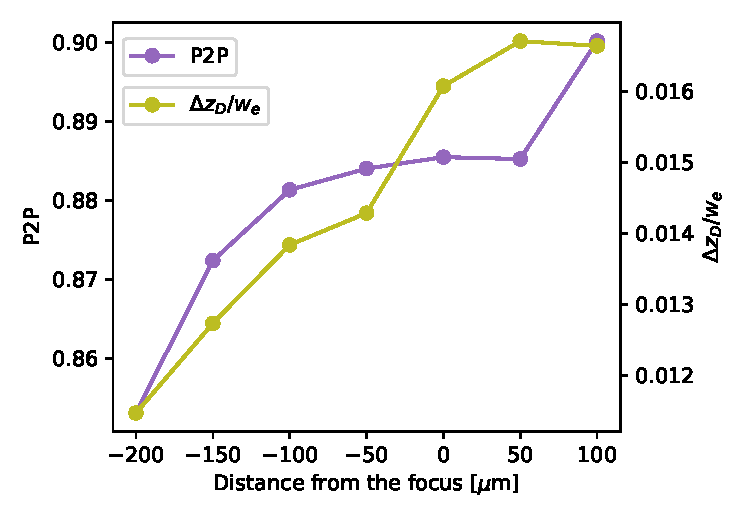
\includegraphics[width=\textwidth]{chapters/chapter_3/figures/p2p_focus.pdf}
        \caption{Peak to peak}
        \label{fig:p2p}
    \end{subfigure}
    \begin{subfigure}{0.5\textwidth}
        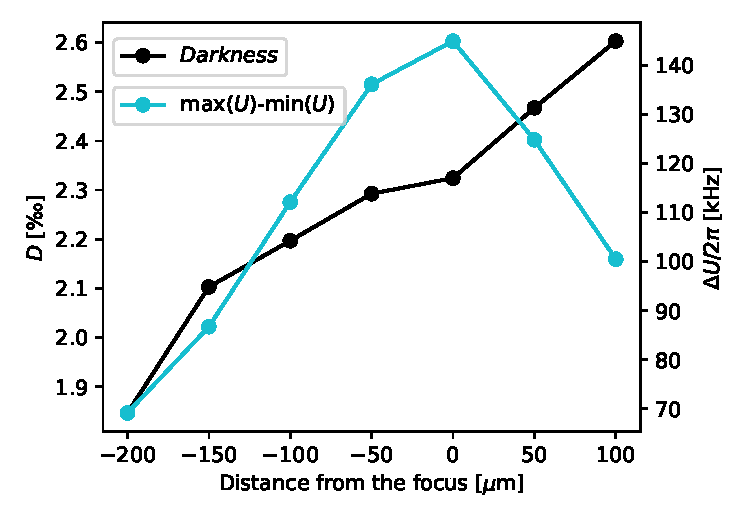
\includegraphics[width=\textwidth]{chapters/chapter_3/figures/darkenss_focus.pdf}
        \caption{Darkness and effective potential}
        \label{fig:focus_darkenss}
    \end{subfigure}\\

    \begin{subfigure}{0.5\textwidth}
        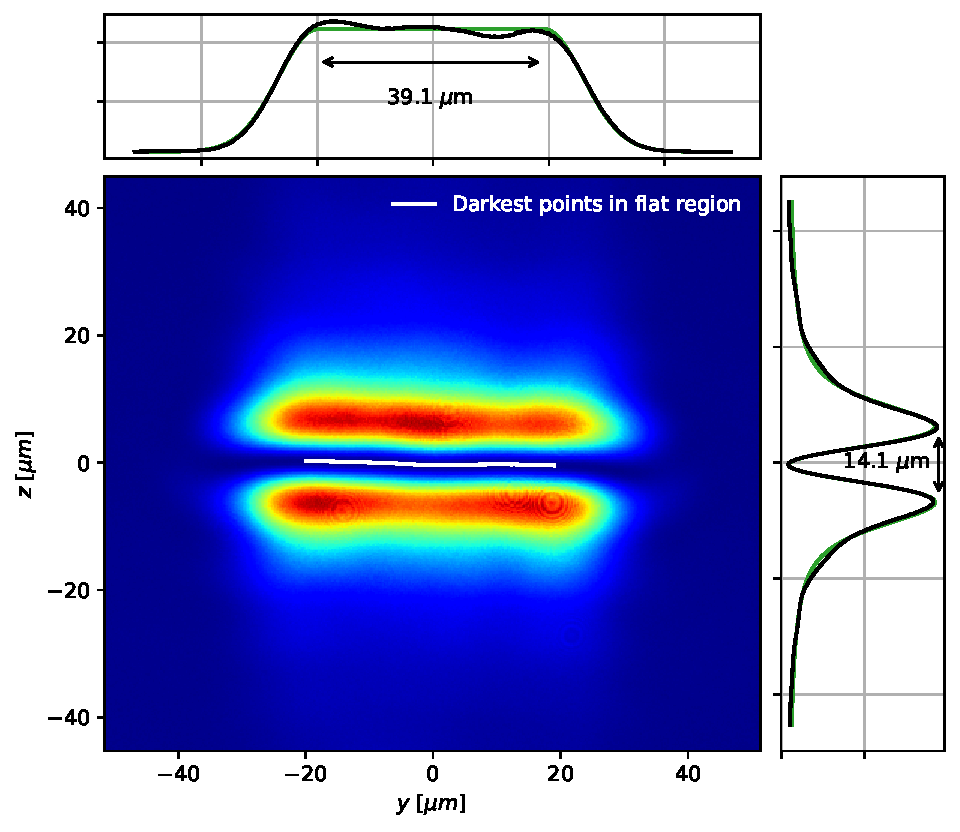
\includegraphics[width=\textwidth]{chapters/chapter_3/figures/focused_anal.pdf}
        \caption{Focused image}
        \label{fig:focus_image}
    \end{subfigure}
    \begin{subfigure}{0.5\textwidth}
        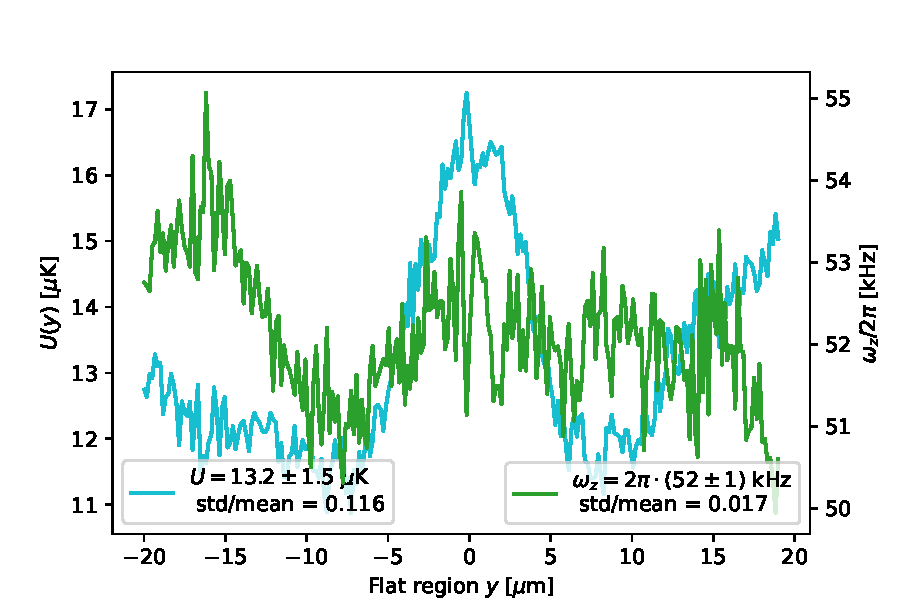
\includegraphics[width=\textwidth]{chapters/chapter_3/figures/omega_U_5focus.pdf}
        \caption{Trapping frequency and effective potential}
        \label{fig:focus_U_omega}
    \end{subfigure}
    \caption{Analysis of the images across the focus for a beam with a diameter of \SI{5.0}{mm}. The images (a)-(d) show the dependency of various parameters on the distance from the focus. Picture (e) shows the focused image and picture (f) the variation of the trapping frequency and the effective potential along the $y$ direction for the focused image.}
    \label{fig:analysis_focus}
\end{figure}

First, we computed the characteristic sizes of the light sheets, namely the length of the flat region $2w_F$ and the distance between the peaks $2w_e$. The result is shown in \cref{fig:focus_size}. We notice that the peak distance is minimized for a particular position of the imaging system, which we identified as the focus. On the other hand, the length of the flat region seems to grow linearly while moving along the focus. Then we shifted our attention to the trapping frequency $\omega_z$ and its relative variation along the $y$ direction $\Delta \omega_z/\omega_z$, where $\Delta \omega_z$ is the standard deviation of the trapping frequency over different points $y$. The trapping frequency $\omega_z$ was calculated using the overexposed images for higher resolution. The result, shown in \cref{fig:focus_omega}, confirms that the focus is well-defined, since at that point $\omega_z$ is maximal and its variation minimal. We also computed the average darkness $D$ (\cref{eq:darkness}), shown in \cref{fig:focus_darkenss}. From the plot, we notice that the darkness increases along the focus. This means that the closer to the phase plate we look, the darker the central region is. This is compatible with the assumption that the darkest point is limited by some background noise. Then $D$ is only given by the peak intensity, which is inversely proportional to $w_F$.

To evaluate the uniformity of the light sheet, we computed three parameters. The first is the P2P, defined before in \cref{eq:p2p} and plotted in \cref{fig:p2p}. We notice that it seems to grow, approaching one, while moving away from the focus in the positive direction. This would indicate an intensity distribution that gets more uniform far from the focal point in one direction and less uniform in the opposite direction. Another way to look at the uniformity of the distribution is to look at the position of the darkest point in the central region. These points are shown in \cref{fig:focus_image} as a white line for the focused image. The standard variation $\Delta z_D$ of their $z$ coordinate, calculated along the $y$ direction, is reported in \cref{fig:p2p}, scaled by $w_e$. We notice that the uniformity evaluated in this way has an opposite behaviour compared to the P2P. In fact, the further we move away from the focus in the direction that maximizes the P2P, the more the vertical position of the darkest points varies. This implies that the atoms would not move in a straight line, but they would follow an irregular path. However, if the trap is tight enough and this degree of freedom is frozen, the motion should not matter for the physics of the experiment. The third parameter used to evaluate the uniformity of the light sheet is the difference $\Delta U$ between the highest and the lowest effective potential felt by the atoms in the flat region aloong the nodal line, as defined in \cref{eq:effectivr_potential}. Surprisingly, this difference has a maximum at the focal point. It is also interesting to notice that it has an order of magnitude of \SI{5}{\micro K}, not negligible compared to the energies involved in our system. An example of the trend of $U(y)$ and $\omega_z(y)$ along the $y$ direction for the focused image is also presented in \cref{fig:focus_U_omega}.


\subsubsection{Analysis of the focused images}
After analysing the behaviour of the phase plate at different distances from the focus, we shifted our attention to the influence of the beam size. For this, we only considered focused images (fifth row of \cref{fig:grid}). For these images, we computed the same quantities as above.
The results are shown in \cref{fig:analysis_diam}.

The characteristic dimensions of the light sheet $w_F$ and $w_e$ can be observed in \cref{fig:diam_size}. We notice that  the length of the flat region increases with the diameter of the beam, going from a minimum of around \SI{30}{\micro m} for a beam of \SI{4.8}{mm} to a maximum of around \SI{45}{\micro m} for a beam of \SI{5.5}{mm}. This size should be compared with an expected width of \SI{40}{\micro m} for a beam of \SI{6}{mm}. On the other hand, the distance between the two peaks in the $z$ direction shows an opposite behaviour, decreasing with the increase of the beam diameter.

The behaviour of the trapping frequency, shown in \cref{fig:diam_trap}, also shows a clear dependence on the beam diameter. We notice that both its mean value $\omega_z$ and its relative variation $\Delta \omega_z / \omega_z$ increase for bigger beams. Moreover, we observe that for all the tested diameters $\omega_z$ is above $2\pi\cdot\SI{45}{kHz}$, therefore enough to trap the atoms in a 2D space. The dependence of the darkness $D$ (averaged over $y$) is reported in \cref{fig:diam_dark}. In this case, we do not observe a clear relation between this parameter and the beam size. For all the beams, we measure a darkness of the order of 4-5~‰. This suggests that to optimize the darkness the alignment of the setup is more important than the size of the beam.

The uniformity of the light sheet could be evaluated looking at the P2P, at the variation of the position of the darkest points $\Delta z_D$ and at the difference $\Delta U$. The first two parameters clearly show a higher flatness for smaller beams, with a smaller variation $\Delta z_D / w_e$ and a P2P closer to one. This is also in agreement with what was observed for the trapping frequency, whose variation was smaller for smaller beams. The data for the potential difference $\Delta U$ is less clear, but still compatible with the same conclusions. In particular, we notice that the potential variation is of the order of \SI{10}{\micro K}, so not negligible if compared to the energies involved in the system.

\begin{figure}
    \begin{subfigure}{0.5\textwidth}
        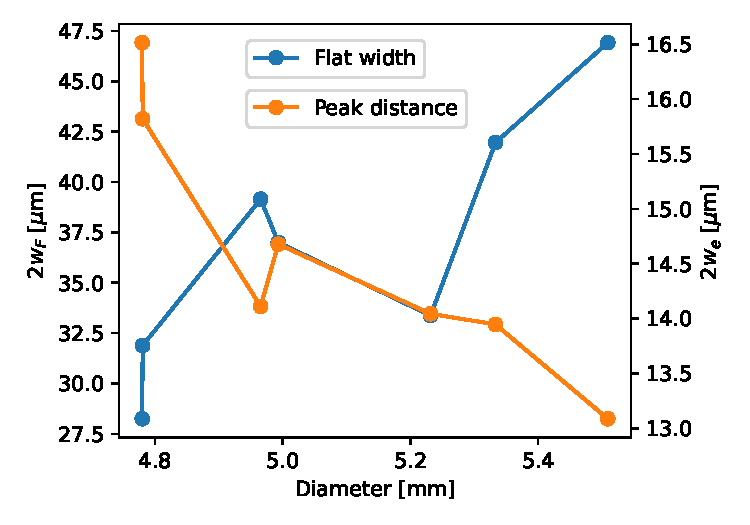
\includegraphics[width=\textwidth]{chapters/chapter_3/figures/size.pdf}
        \caption{Size}
        \label{fig:diam_size}
    \end{subfigure}
    \begin{subfigure}{0.5\textwidth}
        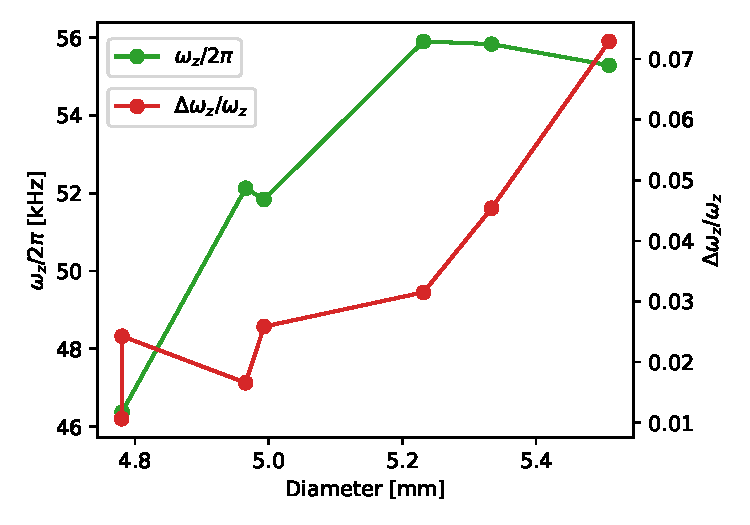
\includegraphics[width=\textwidth]{chapters/chapter_3/figures/trapp_freq.pdf}
        \caption{Trapping frequency}
        \label{fig:diam_trap}
    \end{subfigure}\\

    \begin{subfigure}{0.5\textwidth}
        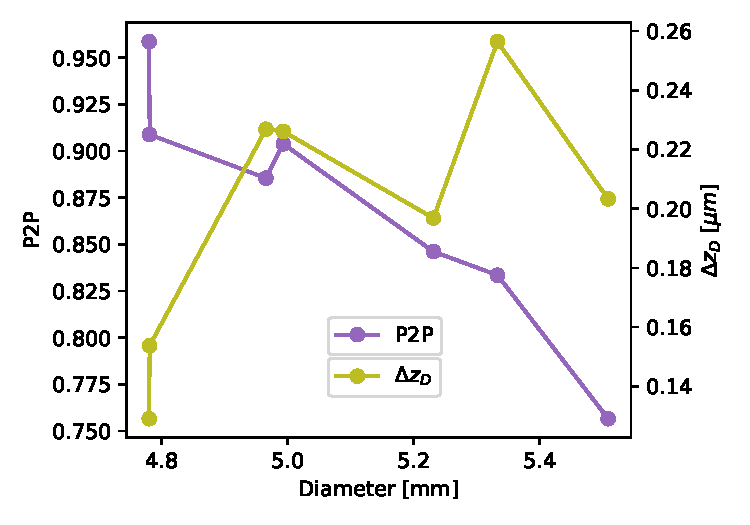
\includegraphics[width=\textwidth]{chapters/chapter_3/figures/p2p.pdf}
        \caption{Peak to peak}
    \end{subfigure}
    \begin{subfigure}{0.5\textwidth}
        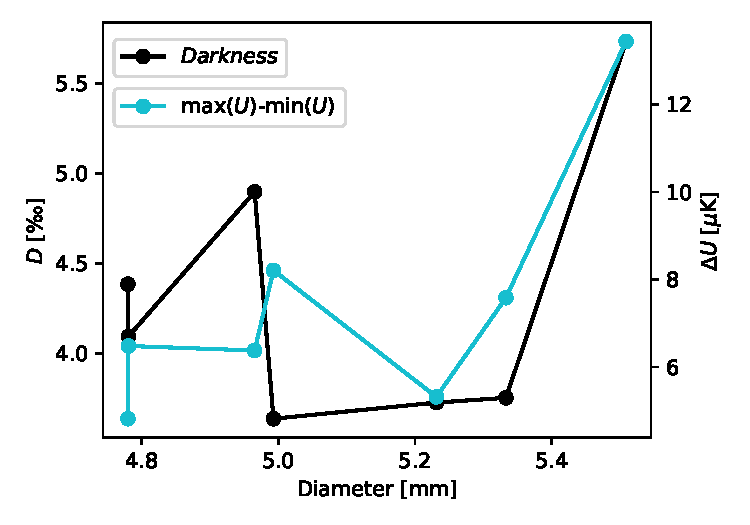
\includegraphics[width=\textwidth]{chapters/chapter_3/figures/darkenss.pdf}
        \caption{Darkness and effective potential}
        \label{fig:diam_dark}
    \end{subfigure}
    \caption{Analysis of the focused images for different sizes of the input beam.}
    \label{fig:analysis_diam}
\end{figure}

\subsection{Additional considerations}
Before concluding the report, we present some smaller findings that have proven to be interesting during the characterization process. It may be useful to take them into account when trying to build and align the final setup.

\subsubsection{Alignment of the phase plate}
In order to characterize the phase plate, the setup had to be correctly aligned. The most important alignment procedure was assuring that the beam hit the centre of the phase plate, in particular in the vertical direction. An incorrect alignment resulted in a central region with bright areas, that would suppress the transport of the atoms.

To align the phase plate, the intensity distribution was observed with a camera set with a long exposure time. Most of the pixels of the resulting image were saturated, but not the ones in the central region. Acting on a screw that moves the phase plate vertically, it is possible to optimize the darkness in the central region. An example of aligned and misaligned phase plates is presented in \cref{fig:alignment}.
\begin{figure}
    \begin{subfigure}{0.3\textwidth}
        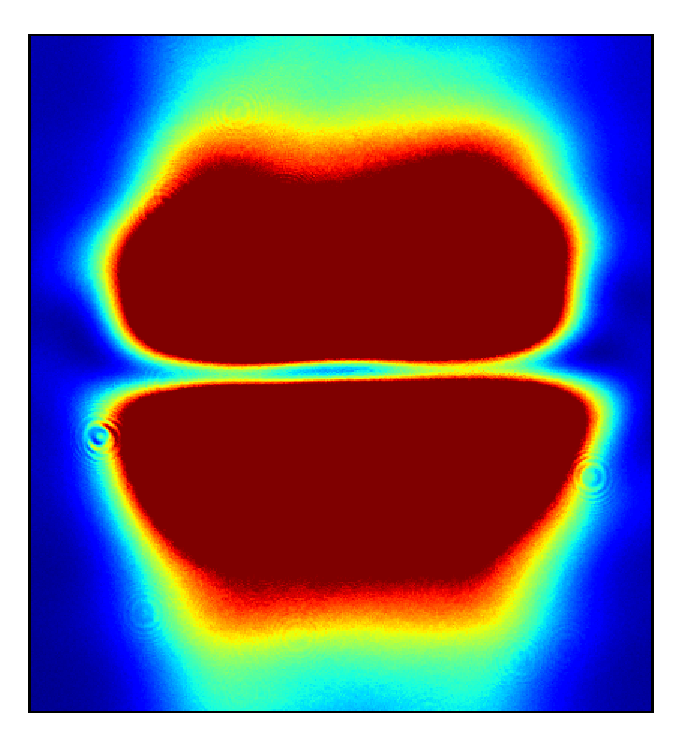
\includegraphics[width=\textwidth]{chapters/chapter_3/figures/align1.pdf}
        \caption{Misaligned}
    \end{subfigure}
    \hfill
    \begin{subfigure}{0.3\textwidth}
        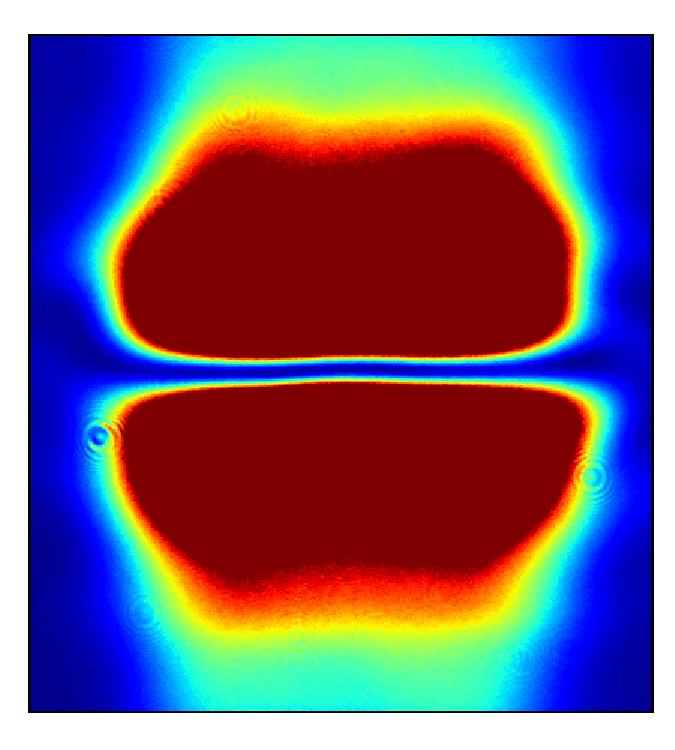
\includegraphics[width=\textwidth]{chapters/chapter_3/figures/align3.pdf}
        \caption{Aligned}
    \end{subfigure}
    \hfill
    \begin{subfigure}{0.3\textwidth}
        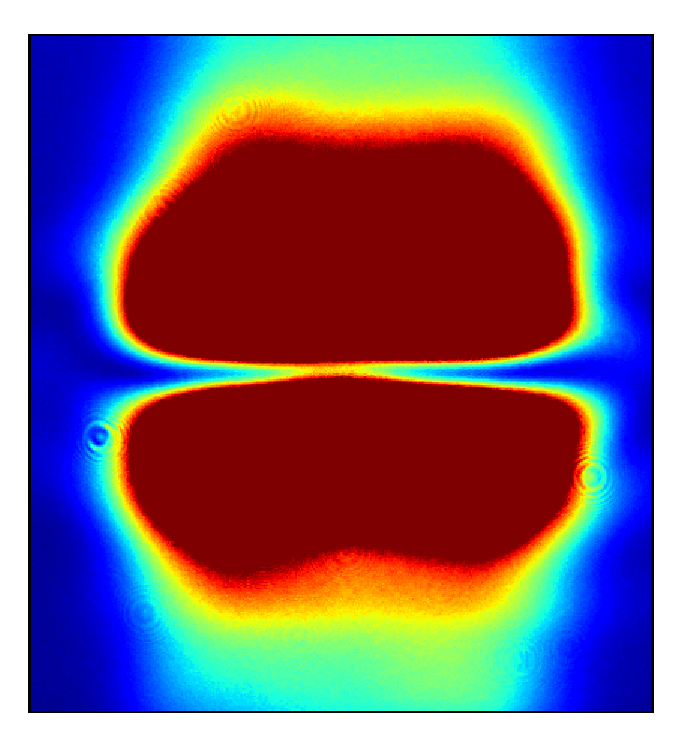
\includegraphics[width=\textwidth]{chapters/chapter_3/figures/align2.pdf}
        \caption{Misaligned}
    \end{subfigure}
    \caption{The vertical alignment of the phase plate is performed looking a saturated picture and optimizing the darkness at the centre.}
    \label{fig:alignment}
\end{figure}

\subsubsection{Singlet or achromatic focusing lens}
It was found that the quality of the focusing lens placed after the phase plate is essential for the final result. In particular, we compared the use of a singlet lens and of an achromatic lens. Both lenses had the same focal length of \SI{100}{mm} and the beam incident on the phase plate was also the same. The result is displayed in \cref{fig:sing_achr}. It is clear that the use of an achromatic lens greatly improves the result. The intensity distribution obtained with the achromatic lens is more uniform ($\text{P2P} = 0.86$), compared to the one generated by the singlet lens ($\text{P2P} =0.76$).
\begin{figure}
    \centering
    \begin{subfigure}{0.45\textwidth}
        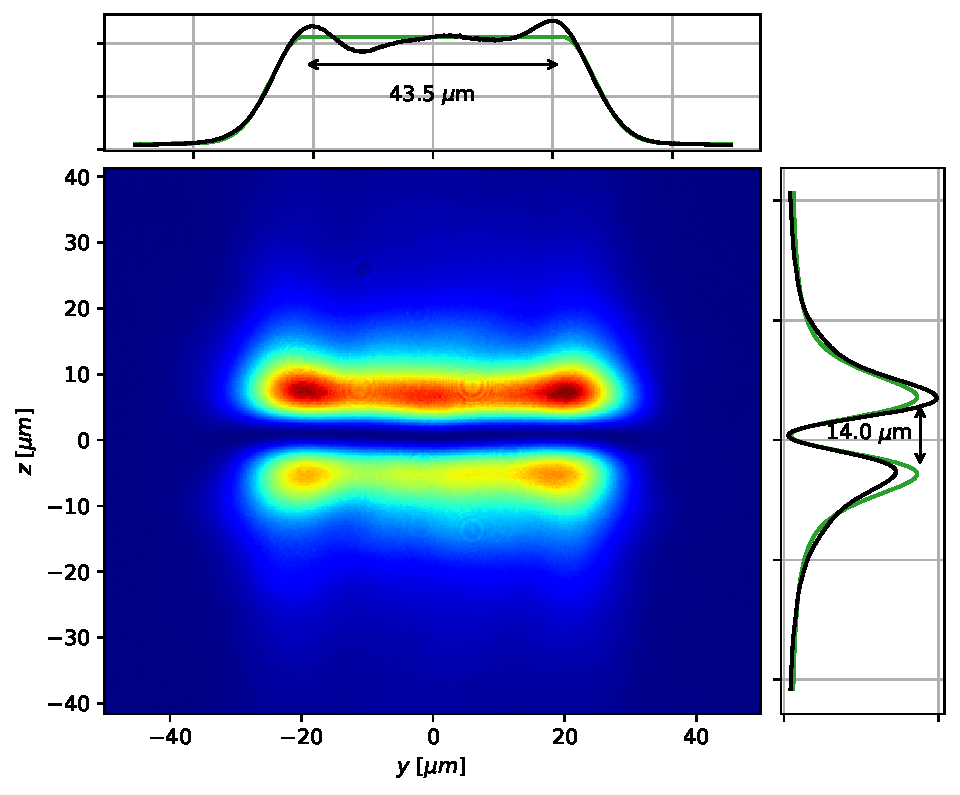
\includegraphics[width=\textwidth]{chapters/chapter_3/figures/sing.pdf}
        \caption{Singlet lens}
        \label{fig:singlet}
    \end{subfigure}
    \hfill
    \begin{subfigure}{0.45\textwidth}
        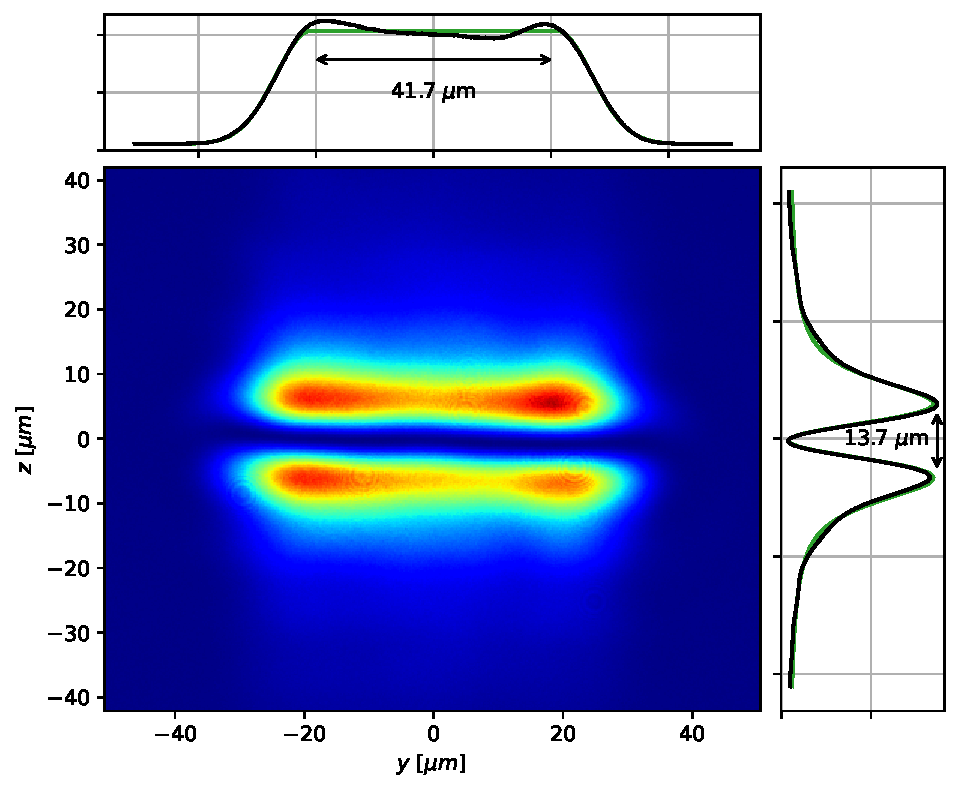
\includegraphics[width=\textwidth]{chapters/chapter_3/figures/achr.pdf}
        \caption{Achromatic lens}
        \label{fig:achr}
    \end{subfigure}
    \caption{Intensity distribution for the same beam, but using two different lenses after the phase plate. The first lens (a) is a singlet lens and the second (b) an achromatic lens.}
    \label{fig:sing_achr}
\end{figure}

\subsubsection{Use of a pinhole in the telescope}

\begin{figure}
    \centering
    \begin{subfigure}{0.45\textwidth}
        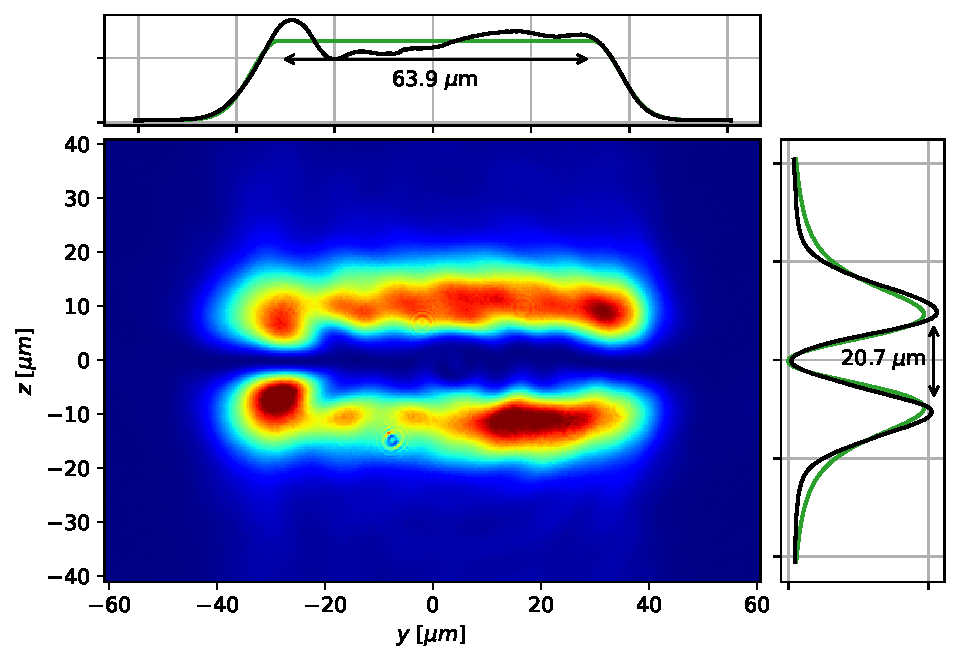
\includegraphics[width=\textwidth]{chapters/chapter_3/figures/large_nopin.pdf}
        \caption{\SI{6}{mm}, without pinhole}
    \end{subfigure}
    \hfill
    \begin{subfigure}{0.45\textwidth}
        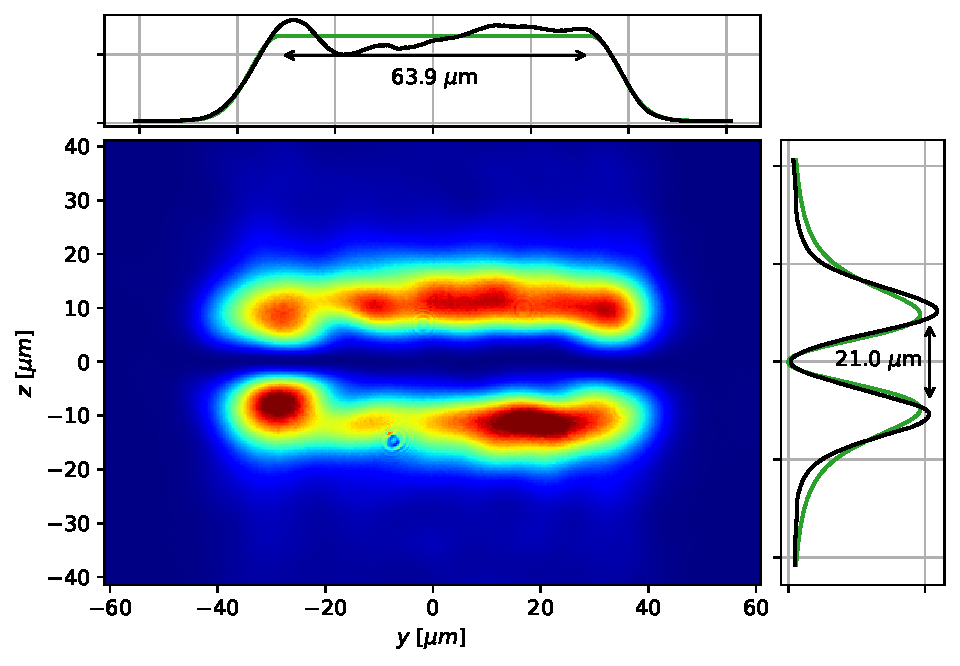
\includegraphics[width=\textwidth]{chapters/chapter_3/figures/large_pin.pdf}
        \caption{\SI{6}{mm}, with pinhole}
    \end{subfigure}\\
    \vspace{0.3cm}
    \begin{subfigure}{0.45\textwidth}
        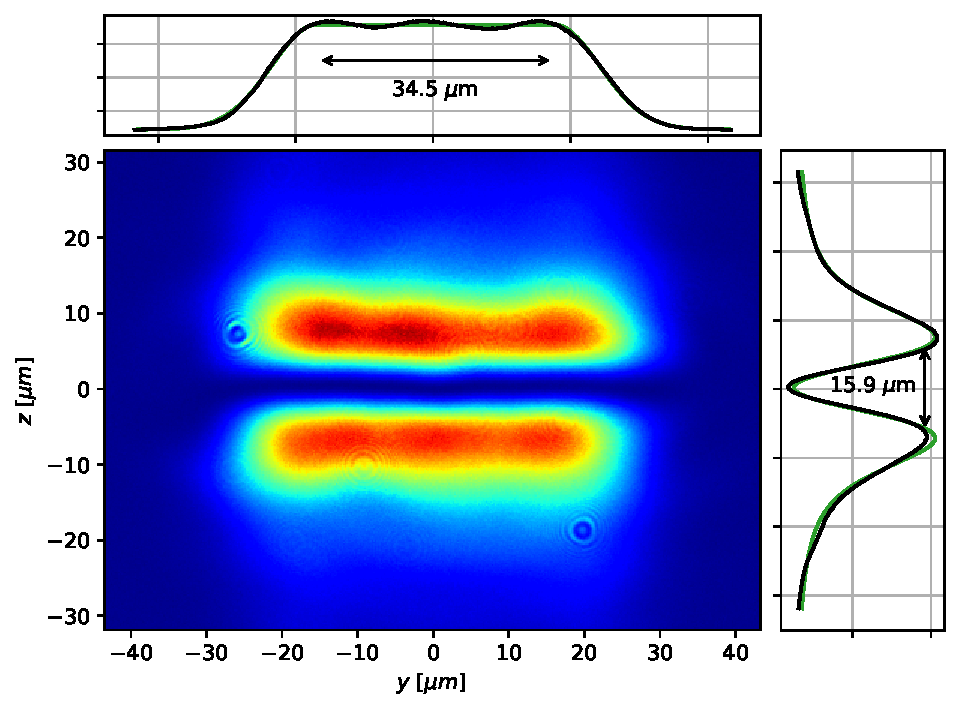
\includegraphics[width=\textwidth]{chapters/chapter_3/figures/small_nopin.pdf}
        \caption{\SI{5}{mm}, without pinhole}
    \end{subfigure}
    \hfill
    \begin{subfigure}{0.45\textwidth}
        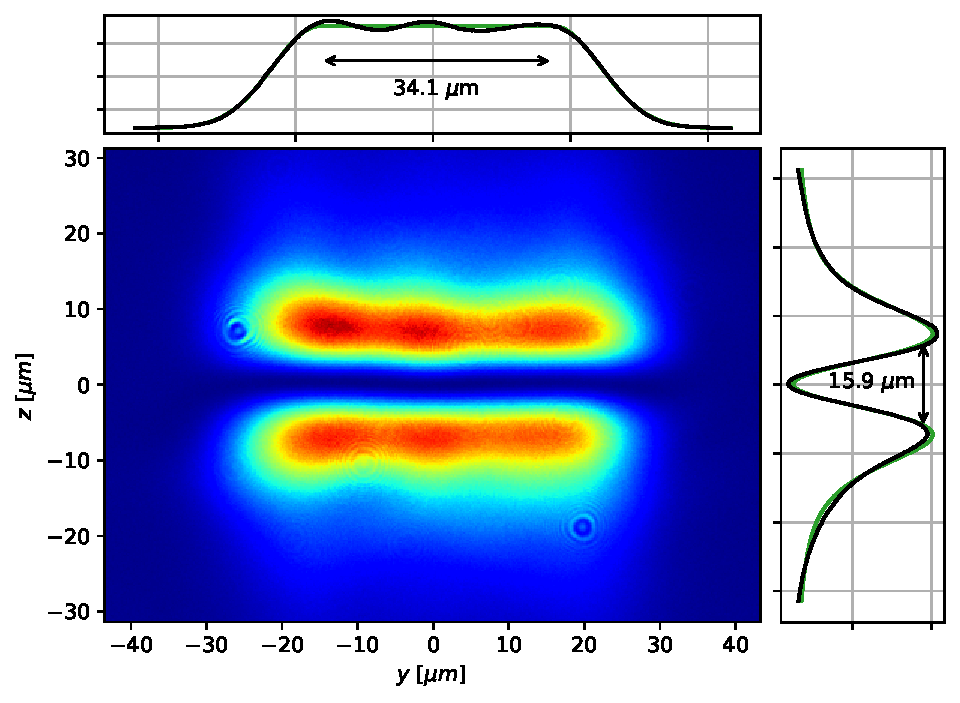
\includegraphics[width=\textwidth]{chapters/chapter_3/figures/small_pin.pdf}
        \caption{\SI{5}{mm}, with pinhole}
    \end{subfigure}
    \caption{Influence of the use of a pinhole in the telescope $-50/150$ for two beam sizes.}
    \label{fig:pin}
\end{figure}

In order to try to reduce the aberrations introduced by the telescope, the usage of a pinhole placed between the two lenses was investigated for small and large beams. In \cref{fig:pin} we present the result for the $-50/150$ telescope. It is important to notice that since the first lens is a diverging lens, the pinhole is almost completely open, and in fact partially \enquote{cuts} the beam. However, even in this unusual configuration, the pinhole seems to have an effect. In particular, as it can be observed from the figures, the use of the pinhole reduces spherical aberrations and contributes improving the final result, especially for larger beams. On the other hand, for beams close to the desired size (around \SI{5}{mm}), it does not seem to have a huge impact on the final intensity distribution.

\subsubsection{Fixing the horizontal dark line}
In \cref{sec:characterization_methods} it was explained how we computed the quantities used to characterize the phase plate. In particular, for quantities like the trapping frequency and the darkenss, we fitted a parabola along the $z$ direction for every point in the $y$ direction, and extracted the dependency of the parameters on $y$ (e.g. $\omega_z(y)$, $D(y)$ \dots). For this process, the parabolic function used in the fit had three free parameters, namely the three coefficients of a second order polynomial. This means that the vertex of the parabola was allowed to have an arbitrary height (used to compute the darkness $D$) and position (used to compute $\Delta z_D$).

\begin{figure}
    \centering
    \hfill
    \begin{subfigure}{0.4\textwidth}
        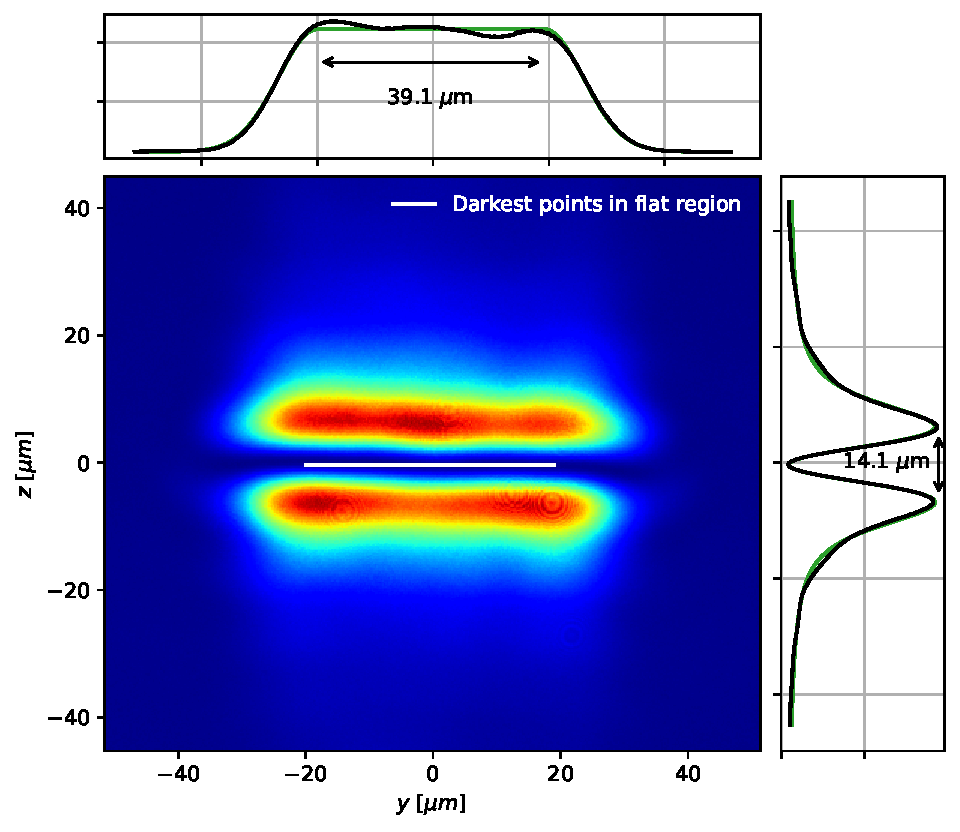
\includegraphics[width=\textwidth]{chapters/chapter_3/figures/fixedline.pdf}
        \caption{Intensity distribution}
        \label{fig:int_fixedline}
    \end{subfigure}
    \hfill
    \begin{subfigure}{0.5\textwidth}
        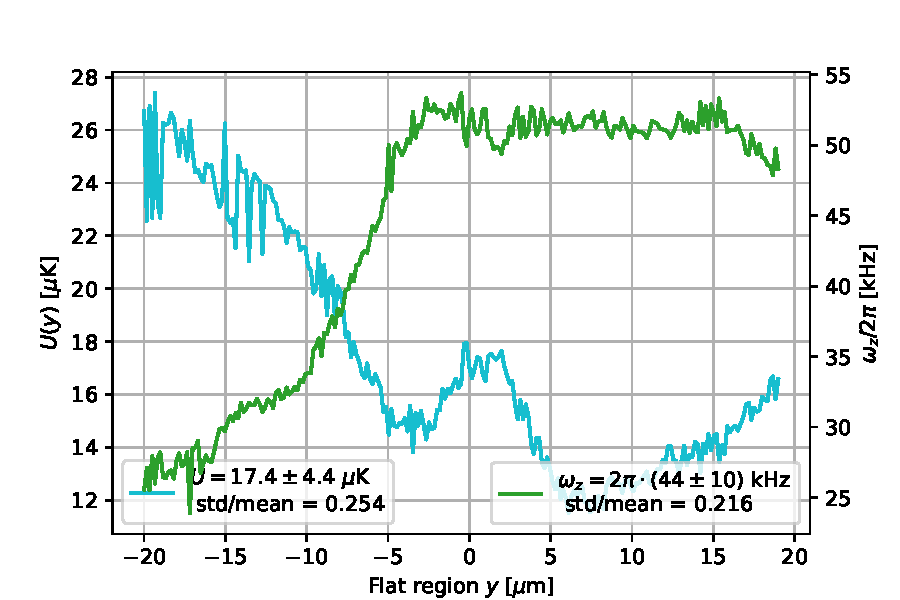
\includegraphics[width=\textwidth]{chapters/chapter_3/figures/trap_fixedline.pdf}
        \caption{Trapping frequency and effective potential}
        \label{fig:trap_fixedline}
    \end{subfigure}
    \hfill
    \caption{Analysis of the focused image for a \SI{5}{mm} beam keeping the coordinate of the position of the dark central region fixed. The result should be compared to \cref{fig:focus_image,fig:focus_U_omega}.}
    \label{fig:fixedline}
\end{figure}

Another possible approach is to fix the $z$ position of the vertex $z_D$, and fit a function with only two free parameters. In this case, it is logical to set $z_D$ to the position of the minimum of the integrated intensity $I_y(z)$, found by fitting the distribution $I_\text{th}(z)$ (cf. \cref{sec:characterization_methods}). The result is shown in \cref{fig:fixedline}. We notice that the irregularity of the intensity is moved from a variation in the $z$ coordinate of the minima to a bigger variation of the trapping frequency and effective potential along the $y$ direction. In particular, both the trapping frequency and the effective potential show variations larger than a factor of two (between \SI{25}{kHz} and \SI{50}{kHz} for $\omega_z$ and between \SI{12}{\micro K} and \SI{26}{\micro K} for $U$). We consider this method inferior to the one described above, since in reality the atoms would move in the region of lower potential, so following an irregular path, rather than in a straight line. The effective potential felt by the atoms would be the one calculated in the previous section, and not the one found fixing $z_D$.

